
\chapter{When? Dark Matter production mechanisms}\label{chapter:production}
In this section we summarize the main cosmological mechanisms that can produce the observed DM abundance, eq.~(\ref{eq:OmegaDMh2}).

Section~\ref{sec:thermal_relic} discusses DM as a thermal relic (freeze-out). 
This is often considered to be the most plausible mechanism for DM production, and is certainly the one that has been the most popular in the community for the past few decades. 
As we will elaborate below, its appeal is twofold: 
i) the only assumption needed is a `feebly' interacting stable particle in the primordial thermal bath;
ii) this assumption fits well with a number of particle physics theories beyond the Standard Model (BSM),
such as SuperSymmetry. The second point is arguably losing some of its attractiveness, because the other, more strongly interacting BSM particles, which are also predicted in such theories, have not yet showed up in any of the searches. The first point, however, still stands strong. 
Historically, the freeze-out mechanism has been considered predominantly for particles interacting with the weak force of the SM. More recently, however, it has been extended to particles interacting with other (feeble) forces.

Section~\ref{sec:freeze-in} discusses the freeze-in mechanism and some of its variants. As we will see below, this mechanism is quite opposite in spirit to the freeze-out, since it assumes that DM particles are completely absent from the primordial thermal bath. It does, however, also provides a natural paradigm to explain the abundance of DM in terms of a few measurable particle physics properties.

Section \ref{sec:inflDMprod} deals with mechanisms that may play a role in the inflationary phase of the Universe's evolution.
In particular, section~\ref{sec:infl} discusses DM production directly from the decay of the inflaton field. 
Section~\ref{sec:misalignement} shows how ultra-light DM can be produced from an initial scalar condensate.

Section~\ref{sec:asymmetricDM} discusses Asymmetric DM. The attractiveness of this mechanism is that it parallels the presumed production mechanism of ordinary matter, i.e.,~baryogenesis, thereby potentially providing a natural reason for why the dark and ordinary matter abundances are comparable in size. On the other hand, while many ideas for baryogenesis have been put forward, experimentally, the full set of ingredients for a successful baryogenesis theory has not been yet discovered.

Finally,  section~\ref{sec:DMprodPT} reviews briefly the DM production mechanisms that feature phase transitions, while  section~\ref{sec:PBHform} describes the production of primordial black hole DM.

\medskip

Notice that most if not all of the production mechanisms require DM to have some interactions with the ordinary matter and/or with itself, beyond just gravity.  
These interactions need to be weak enough to satisfy the `non-interacting' bounds discussed in section~\ref{sec:DMparticle}. 
Still, as we already mentioned above, the existence of such interactions is not required observatonally in any way by the cosmological and astrophysical evidences discussed in chapter \ref{sec:evidences}.

\medskip

Before presenting the various DM production mechanisms, it is useful to introduce a quantity, which expresses DM density
in a form most useful for cosmological computations.
The use of number density $n_{\rm DM} = \rho_{\rm DM}/M$ has two `drawbacks': it depends on the unknown DM mass $M$, and evolves significantly during the cosmological history, i.e., it is a function of  time $t$ (or, equivalently, a function of temperature $T)$.
Ratios such as $n_{\rm DM}/n_\gamma$ evolve less. 
However, photons do have their own cosmological history, getting periodically 
heated by the annihilations of charged particles when these become non-relativistic.
A more useful quantity to measure the cosmological abundance of DM
 is instead
\beq \label{eq:YDMdef}
 Y_{\rm DM}(T) \equiv  \frac{n_{\rm DM}(T)}{s(T)},
 \eeq
where $s = 2\pi^2 g_{s}(T) \, T^3/45$ is the total entropy density. Its present day value $s_0$ follows from $T_0 = 2.725\,{\rm K}$ and $g_{s0} = {43}/{11}$.\footnote{Entropy is discussed in appendix~\ref{app:Cosmology};
the effective number of total degrees of freedom 
$g_{\rm s}(T)$ is plotted for the SM in  fig.\fig{dofSM} and equals $106.75$ at temperatures much above the weak scale.}
The total entropy in a comoving volume $V$, $S = s V$, 
is conserved during the cosmological evolution as long as  thermal equilibrium holds. 
The quantity $Y_{\rm DM}(T)$ is therefore very convenient, since it stays constant during most of the cosmological history,
whenever the number of DM particles per comoving volume is conserved.
This is in particular the case at late times when DM is decoupled, and at early times when DM was  possibly in a thermal equilibrium with the SM thermal bath.
\label{DM cosmological abundance}


Its present day value
$Y_{\rm DM 0} = Y_{\rm DM}(T_0)$
is linked to the DM mass density $\Omega_{\rm DM}$ as
\beq 
\label{eq:OmegaDMY}
\Omega_{\rm DM} = \frac{\rho_{\rm DM}}{\rho_{\rm cr}} =\frac{s_0Y_{\rm DM0}  M}{3H_0^2/8\pi G} 
= \frac{688 \pi^3 \, T_0^3 \, Y_{\rm DM 0} \, M}{1485 \, M_{\rm Pl}^2 \, H_0^2}.
\eeq
Inserting the present Hubble constant $H_0 = h\times 100\km/{\rm sec\cdot Mpc}$, we obtain
\beq \index{DM abundance!cosmological}
\label{eq:YDM0}
\bbox{Y_{\rm DM0} = \frac{0.44\eV}{M}
\frac{\Omega_{\rm DM} h^2 }{0.120}}. 
\eeq

Let us first assume that DM decoupled from the thermal bath while it was still relativistic,\footnote{The analogous neutrino decoupling is discussed in section~\ref{neutrinoDM}.} which then gives $Y_{\rm DM0} = n_{\rm DM}/s = 45 \, \zeta(3)/2 \pi^4 \times g_{\rm DM}/g_{\rm s}(T_{\rm dec})$,
with $g_{\rm s}(T_{\rm dec})\circa{<}100$ the number of SM degrees of freedom at the time of DM decoupling. Here we are using eq.~(\ref{eq:relativisticquantities}) in appendix~\ref{app:Cosmology}, and assuming for definiteness the Fermi-Dirac distributed DM (the bosonic case gives a result that differs just by an $\mathcal{O}(1)$ factor). 
In this case DM abundance is reproduced for
 $M \approx 1.6 \eV\, g_{\rm s}(T_{\rm dec})/g_{\rm DM}$,
  i.e., a thermal freeze-out of relativistic DM results in a hot or warm DM, which is highly disfavored by observations, as discussed in section~\ref{sec:WarmDM}.\footnote{Relativistic freeze-out of DM  
can give heavy enough DM, if it happens in a hypothetical `dark sector' that is decoupled from the SM and also has a lower temperature~\cite{DMrelFO}. This could for instance happen if the inflaton dominantly  decays into the SM sector.
In such a case, DM could even just be a free particle that does not undergo any freeze-out.} 
In order to obtain cold DM, one needs $M\circa{>}{\rm keV}$, and as a consequence a DM number density that is small or very small: $Y_{\rm DM0} \ll 1$.
As discussed in the next section, the non-relativistic decoupling satisfies this requirement.





\section{DM as a thermal relic}\label{sec:thermal_relic} 
\index{Freeze-out}\index{DM cosmological abundance!freeze-out}\index{DM!as weak-scale particles}
The freeze-out mechanism~\cite{cosmobooks,DMFO} assumes that DM is a stable particle with mass $M$, 
which in the early Universe had interactions with the SM particles that were faster than the Hubble rate.
DM was thus a component in the thermal bath, with the SM and DM sectors thermalised to a common temperature $T$, maximising the entropy. In the absence of a conserved DM number, thermalization erases any possible primordial inflationary differences in the two components,
so that the same SM/DM fluid filled all the Universe, with common adiabatic inhomogeneities.

DM eventually decoupled: the freeze-out mechanism assumes that the current DM abundance is a left-over (a `relic') of an incomplete (`frozen') process. 
Since the iso-curvature inhomogeneities are not re-generated when thermal equilibrium between the SM and DM 
is lost~\cite{AdiabaticDM}, freeze-out satisfies the observational bound on iso-curvature perturbations in eq.\eq{isocurvaturebound}, which demands the same `adiabatic' pattern of SM and DM inhomogeneities.
\index{DM properties!adiabatic}
\label{DM cosmological abundance!iso-curvature}\label{Iso-curvature}

In the next sections we consider freeze-out for various particle-physics processes that
might have happened.


\subsection{$2\leftrightarrow 0$ annihilations: estimate of the relic abundance}\label{sec:thermalapprox}
Perhaps the most plausible process is annihilations of a pair of DM particles 
(or annihilations of DM and anti-DM) into SM particles.
Introducing a soccer notation we denote this as $2\leftrightarrow 0$, 
enumerating explicitly the number of dark-sector particles in the initial and final states,
summing over both particles and anti-particles.
Any number of SM particles can be present in the initial or final state.
Often the dominant process involves two SM particles in the final state:
\beq 
\hbox{DM DM $\leftrightarrow$ SM SM},\qquad\hbox{where SM denotes any Standard Model particle}.
\eeq
In this section we start sketching the physics involved in this process, providing very rough analytical approximations
that will then be refined in sections~\ref{sec:reliccomputation} and~\ref{analyticapprox}.

\medskip

The typical particle energy at temperature $T$ is $E\sim T$ and the typical de Broglie wavelength is $1/E$, therefore the
number density $n$ and energy density $\rho$ are
\beq n\sim T^3,\qquad \rho\sim T^4, \qquad {\rm for}\quad T\gg M.\eeq
When the temperature of the Universe drops below the DM mass, $M$, 
various processes try to maintain thermal equilibrium. As long as this is maintained, the DM number density follows a Boltzmann-suppressed form
\beq 
\label{eq:Boltzmann:suppress}
n_{\rm DM}\propto e^{-M/T}.
\eeq
Since DM is stable (or so long-lived that its decays play no role), the dominant process that violates the total DM number (assumed not to be conserved, otherwise see section~\ref{sec:asymmetricDM})
are annihilations involving two DM particles, with total cross section $\sigma$.
As the temperature decreases, at some point the DM density becomes so small that the DM DM annihilation rate $\Gamma$ becomes slower than the expansion rate $H$ 
and the thermal equilibrium can no longer be maintained. At this point DM stops annihilating and its abundance {\em freezes out}. This happens when
\beq 
\label{eq:moment_of_fo}
\Gamma \sim \langle n_{\rm DM} \sigma \rangle~ \circa{<} ~H \sim  
\frac{T^2}{M_{\rm Pl}}.
\eeq
On the right hand side, we used $H=\sqrt{8 \pi G_N \, \rho/3}$  with $\rho  \sim T^4$, which is valid for radiation domination
(more precisely $\rho  = \pi^2 g_* T^4/30 \sim T^4$, see Appendix \ref{app:Cosmology}).
For the purposes of these crude estimates, we are neglecting all the numerical factors and keeping only the overall scalings.
Using eq.~(\ref{eq:moment_of_fo}), the out-of-equilibrium DM relic abundance is conveniently estimated in units of the photon number density $n_\gamma \sim T^3$ as
\beq \label{eq:nDMestimate}
\frac{n_{\rm DM}}{n_\gamma} \sim \frac{T_{\rm fo}^2/M_{\rm Pl}\sigma}{T_{\rm fo}^3}\sim
 \frac{1}{M_{\rm Pl} \sigma M},
\eeq
where in the last relation we estimated the freeze-out temperature as $T_{\rm fo} \sim M$, determined by the quick drop in scattering rates for $T/M\lesssim 1$ due to the exponential Boltzmann suppression in \eqref{eq:Boltzmann:suppress}.
The current DM energy density $\rho_{\rm DM}$ is then 
\beq 
\frac{\rho_{\rm DM}}{\rho_{\gamma}}\sim \frac{M}{T_0}
\frac{n_{\rm DM}}{n_{\gamma}} \sim \frac{1}{M_{\rm Pl}\sigma T_0 }  .\label{eq:rhoDMestimate}\eeq
Notice the inverse dependence on the annihilation cross section $\sigma$. As a consequence of it, if there are several stable particles,
the relic density of the universe is dominated by the one with the smallest annihilation cross section ---
the weakest particle wins.

As another very crude approximation, let us put $\rho_{\rm DM} \sim \rho_\gamma$
(it should rather be $\rho_{\rm DM} \sim 1000 \, \rho_\gamma$ today, see fig.\fig{Omegas}, but again we are only focusing on the overall scalings here), 
and the typical expression for the annihilation cross section of a particle with mass $M$
mediated by some light particle with dimension-less coupling $g$, $\sigma\sim g^4/4\pi M^2$, we get
\beq \label{eq:DMrelicmassTeV}
M/g^2\sim\sqrt{T_0 M_{\rm Pl}}\sim\TeV.\eeq
The geometrical average between `zero' (the present temperature $T_0\sim 3\,{\rm K}$)
and `infinity' (the Planck mass $M_{\rm Pl}$)
turns out to be comparable to the energy reached by the present colliders.

\smallskip

The above rough computation shows that a TeV-scale DM particle interacting with $\mathcal{O}(1)$ couplings results in a DM abundance that is roughly equivalent to the one actually observed.
The paradigmatic realization of this kind of DM are WIMPs, Weakly Interacting Massive Particles (see also section~\ref{sec:WIMPs}): weak-scale DM particles that talk to the SM via SU(2)$_{\rm L}$ gauge interactions, controlled by the weak couplings $g \sim g_2\simeq 0.6$, are produced by the thermal freeze-out mechanism in roughly the right amount to explain the observed relic abundance. Historically, this has been dubbed the {\bf `WIMP miracle'}.\index{WIMP!miracle}
In passing, we note that, for the case of TeV-scale DM, eq.\eq{YDM0} implies $Y_{\rm DM0} \simeq 4 \, 10^{-12}$ i.e.~$n_{\rm DM}/n_{\gamma} \sim T_0/M\sim 4 \, 10^{-12}$. This means that DM freeze-out happened at $T_{\rm fo} \sim M/\ln(M/T_0)\sim M/26$, which corrects the above rough approximation.

\smallskip

If  DM annihilation is  mediated instead by some new boson with mass $M' \gg M$,
the interaction becomes an effective dimension-6 operator with coefficient $1/\Lambda^2 \approx g^2/M^{\prime 2}$, and the cross section is $\sigma \sim M^2/4\pi \Lambda^4$. 
The correct DM abundance is now reproduced for
$M \sim \Lambda^2/\TeV$ as long as $M/\Lambda$ is still large enough such that the decoupling happens while DM is already non-relativistic, so that $n_{\rm DM}\ll n_\gamma$.
As discussed in the next section, the non-relativistic limit allows for a simple precise computation.



\subsection{$2\leftrightarrow 0$ annihilations: computation of the relic abundance}
\label{sec:reliccomputation}
As it is clear from the discussion in the previous subsection, the hypothesis that DM is a cold thermal relic fixes the DM annihilation cross section.  
In this subsection we derive its precise value.\index{Boltzmann equation}
The standard tool to perform this kind of cosmological computation is the classical Boltzmann equation
for the DM number density, $dn_{{\rm DM}i}(t,\vec{x},\vec{p})/d^3x\, d^3p$ where $i$ is a superindex that denotes DM polarizations, internal degrees of freedom, etc.
In the early universe, inhomogeneities are at the $10^{-5}$ level so one can neglect them, i.e.,~the $\vec{x}$ dependence in $n$ can be dropped.
Furthermore, scatterings that maintain the kinetic equilibrium are fast enough
that one can assume a Fermi-Dirac or Bose-Einstein distribution in the DM momentum $\vec p$
(both reduce to the Maxwell distribution in the relevant non-relativistic limit).

Hence, one can write a single equation for the total DM number density $n_{\rm DM}(t)$, summed over all DM polarizations, internal degrees of freedom, etc.
This equation has the intuitive form
\beq \frac{1}{a^3} \frac{d(n_{\rm DM} \,a^3)}{dt} = \frac{dn_{\rm DM}}{dt} + 3Hn_{\rm DM} = \langle \sigma v_{\rm rel}\rangle (n_{\rm eq}^2 - n_{\rm DM}^2),
\label{eq:BoltznDM}
\eeq
where $a(t)$ is the scale factor of the universe, $H = \dot a/a$ is the Hubble rate, $n_{\rm eq}$ is the number density that
DM particles would have in thermal equilibrium and $ \langle \sigma v_{\rm rel}\rangle$ is the thermal average of the total annihilation cross section times the relative velocity $v_{\rm rel}$ between annihilating DM particles. 
The term $3Hn_{\rm DM}$ in the expression after the first equality accounts for the dilution of DM density due to the expansion of the Universe.
The two contributions on the right  hand side describe respectively the DM depletion due to annihilations (proportional to $n_{\rm DM}^2$)
and the DM creation via inverse annihilations (proportional to $n^2_{\rm eq}$).
Provided that $ \langle \sigma v_{\rm rel}\rangle$ is  large enough, 
the right hand side expression ensures that DM abundance is in a thermal equilibrium, i.e.,~$n_{\rm DM}=n_{\rm eq}$. 
As the temperature decreases, DM becomes non-relativistic and its equilibrium density is exponentially suppressed: $n_{\rm eq}= g_{\rm DM} (MT/2\pi)^{3/2} e^{-M/T}$.
Here, $g_{\rm DM}$ is the number of degrees of freedom associated with the DM particle ($g_{\rm DM}=1$ for real scalar DM, $g_{\rm DM}=2$ for Majorana fermion DM, etc, see fig. \ref{fig:Omegafreeze-out} right).
Eventually, the DM density becomes so suppressed that the annihilation term fails to keep up with the expansion term (the DM particles are so rare that they are not able to find each other to annihilate), annihilations stop and thus DM decouples.
The observed cosmological abundance of DM is reproduced if thermal equilibrium fails and DM freeze-out occurs at
 $T < T_{\rm fo}\sim M/25$, such that $n_{\rm DM} \approx n_{\rm eq}(T=T_{\rm fo})$. 
 An accurate approximation to the analytic solution of the Boltzmann equation~\cite{DMFO}
 will be derived in section~\ref{analyticapprox}, with the final result given by
\beq \frac{\Omega_{\rm DM} h^2}{0.110} \approx \frac{\sigma v_{\rm cosmo} }{\langle \sigma v_{\rm rel}\rangle_{T\approx M/25}},
\label{eq:OmegaDMapprox}
\eeq
where
\beq
\label{eq:sigmavcosmo}
\bbox{
\sigma v_{\rm cosmo} \approx  
2.2\times10^{-26}\frac{\cm^3}{{\rm s}}=
\frac{1}{(23.0\TeV)^2} \approx 0.73\pb = 0.73~10^{-36}\cm^2.} 
\eeq
The precise numerical result for the special value $\sigma v_{\rm cosmo} $, which reproduces the
cosmological DM abundance, is plotted in fig.\fig{Omegafreeze-out} as a function of $M$.
Another way of stating the `WIMP miracle'  is that the required $\sigma v_{\rm cosmo}$
turns out to `miraculously' correspond to a typical weak annihilation cross section, $\sigma\sim g_2^4/4\pi\, {\rm TeV}^2$.
In more detail, however, this `miracle' does need a TeV energy, i.e., an order of magnitude above $M_{W,Z,h}\sim 100\GeV$.


\medskip

Notice that $\sigma$ is averaged over the various DM components.
This leads to factors of 2 that can generate confusion.
If DM is a real particle (e.g.\ a Majorana fermion) $\sigma$ is given by the usual definition of a cross section ---
averaged over initial polarisations and summed over final states.
A factor of 2 on the right hand side of eq.\eq{BoltznDM}, present because 2 DM disappear in each annihilation, is canceled
by the initial state symmetry factor $1/2$.

If DM is a complex particle (e.g.\ a Dirac fermion) then $n \equiv n_{\rm DM} + n_{\overline{\rm DM}}$.
Here we assume that there is no asymmetry, so that $n_{\rm DM} = n_{\overline{\rm DM}}$.
The average over the 4 possible  initial states is
$\sigma \equiv \frac{1}{4}(2\sigma_{{\rm DM}\,\overline{\rm DM}} + 
\sigma_{\rm DM~DM} + \sigma_{\overline{\rm DM}~\overline{\rm DM}})$.
In many models only ${\rm DM}\,\overline{\rm DM}$ annihilations are present, giving
$\sigma =  \frac12 \sigma_{{\rm DM}\,\overline{\rm DM}}$.
This discussion can be extended, to deal with
more complicated situations where multiple DM states are present,
e.g.,\ degenerate weak-multiplets containing both real and complex components.
Concrete examples are given in section~\ref{models}.




\begin{figure}[t]
$$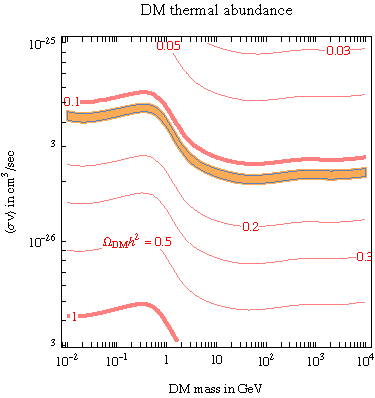
\includegraphics[width=0.47\textwidth]{figs/Omegafreeze-out}\qquad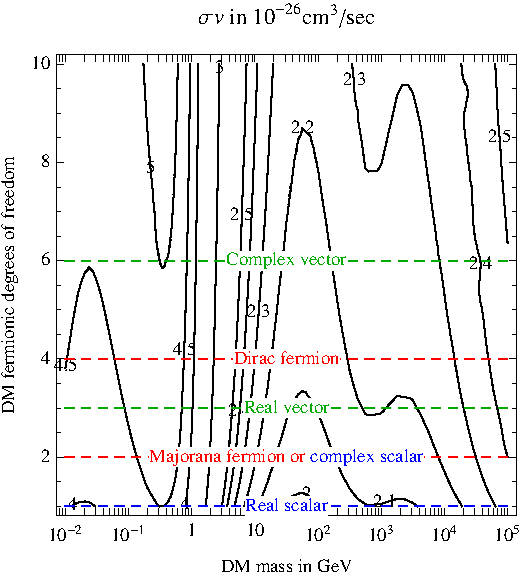
\includegraphics[width=0.44\textwidth]{figs/Omegafreeze-out-dof}$$
\caption[Sample of DM freeze-out]{\em  \label{fig:Omegafreeze-out} 
 {\bfseries Left}: DM freeze-out abundance $\Omega_{\rm DM} h^2$ as function of the DM mass  and of the DM annihilation cross section
 $\langle \sigma v\rangle$ for Majorana DM.
 The measured cosmological DM abundance $\Omega_{\rm DM}h^2 = \OmegaDMexp$, eq.~(\ref{eq:OmegaDMh2}), is reproduced within the orange band at 3 standard deviations. For smaller (larger) annihilation cross sections, i.e.~in the lower (upper) part of the plot, the freeze-out happens too early (too late) and therefore the DM relic abundance is too high (too low).
 {\bfseries Right}: Iso-contours of  the annihilation cross section 
$ \sigma v_{\rm rel}$ in $10^{-26}\cm^3/{\rm sec}$ that reproduces the central value
 of the DM cosmological abundance as function of the DM mass and of the number of DM  degrees of freedom.
This cross-section is a target for indirect DM detection searches.}
\end{figure}






\subsection{$2\leftrightarrow 0$ annihilations: analytic approximation}\label{analyticapprox}

In this section we address in more detail the description of the freeze-out process that we qualitatively discussed above.\footnote{
In the computations of this section we always assume that, thanks to DM-SM collisions, DM particles remain in kinetic equilibrium with the SM particles down to temperatures that are (a few orders of magnitude) below the thermal decoupling temperature of DM annihilations. This means that we can then neglect the details of the DM energy distribution and concentrate on the integrated quantity, the total DM number density. If, for any reason, kinetic equilibrium does not hold, then the standard computations are affected (see, e.g.,~\arxivref{1706.07433}{Binder et al.~(2017)} and \arxivref{2103.01944}{Binder et al.~(2021)}~\cite{KineticEquilibrium}). \\
In the rest of this footnote, let us review the basic concepts of the different equilibriums and decouplings. 
The term {\bf thermal (or chemical) equilibrium} refers to the equilibrium between particle species. It is maintained by the balance between DM annihilations into SM particles and the inverse process of SM particles creating DM. 
When thermal equilibrium fails, DM particles {\em thermally} (or {\em chemically}) {\em decouple} from the thermal bath, i.e,.~they freeze-out, as extensively discussed above. 
{\bf Kinetic equilibrium}~\cite{KineticEquilibrium}\index{Kinetic decoupling} refers to the equilibrium in the energy distributions. It is maintained by very frequent elastic scatterings between DM and SM particles (in particular, with the dominant SM radiation fluid), and typically holds even at temperatures well below $T_{\rm fo}$. When the kinetic equilibrium fails, DM particles {\em kinetically decouple}, therefore their final kinetic distribution in general differs from that of the SM particle species. 
The temperature of kinetic decoupling, $T_{\rm kd}$,  can be estimated by imposing 
$\Gamma_{\rm kin} \sim H$ where $H \sim T^2/M_{\rm Pl}$, and
$\Gamma_{\rm kin} \sim \sigma n T/M$ is the rate of DM energy exchange due to scatterings with cross section $\sigma$
on SM particles with number density $n$.
Assuming $n \sim T^3$ (possibly electrons and neutrinos) and $\sigma \sim g^2 g'^2_{\rm DM}T^2/M'^4$, 
where $M'$ is the mass of some mediator that couples with $g$ and $g'_{\rm DM}$ couplings to matter and DM currents, respectively, one obtains  
\beq T_{\rm kd} \sim (M/M_{\rm Pl})^{1/4} M' /\sqrt{g \, g'_{\rm DM}} .\label{eq:Tkindec}\eeq
The temperature of kinetic decoupling is higher (i.e., the decoupling is earlier) the heavier the DM and the mediator are, and the smaller the couplings. For WIMP DM, $M \sim$ TeV, $M'$ is the mass of the $Z,W^\pm$ bosons and $g = g'_{\rm DM} =g$, so $T_{\rm kd} \simeq 10$ MeV, 
a few orders of magnitude below the DM freeze-out temperature $T_{\rm fo} \sim M/25$.}
For this purpose, it is convenient to a) study the evolution of the total DM abundance as a function of a dimensionless parameter
$z\equiv M/T$, which is ${\mathcal O}(1)$ during freeze out\footnote{Or rather ${\mathcal O}(25)$ for weak-scale particles, as seen above.} and which grows with time as $T$ decreases;
b) factor out the overall expansion of the universe by writing equations for $Y_{\rm DM}=n_{\rm DM}/s$,
the DM abundance in units of the entropy density introduced in eq.~(\ref{eq:YDMdef}).
The Boltzmann equation in terms of $Y_{\rm DM}(z)$ is 
(for details see appendix~\ref{Boltzmann}) \index{Boltzmann equation!for freeze-out}
\beq \label{eq:DMboltzY}
sHZz \frac{dY}{dz} =
  -2\gamma_{\rm ann}   \bigg(\frac{Y^2}{Y^{2}_{\rm eq}}-1\bigg),
 \eeq
where the factor $ Z=1/(1+ \frac{1}{3}\frac{d\ln g_{*s}}{d\ln T})$ can often be approximated as 1,
 and  $\gamma_{\rm ann}$ is the space-time density of annihilations in thermal equilibrium,
  summed over initial state and final states and their polarisations.
 Eq.\eq{gamma2} gives $\gamma_{\rm ann}$ in terms of the annihilation cross section $\sigma(s)$.
 One can easily perform numerical calculations or run public codes such 
 as {\tt MicrOMEGAs} \cite{1801.03509}, {\tt DarkSUSY} \cite{1802.03399}, {\tt MadDM} \cite{1804.00044}, {\tt SuperIsoRelic} \cite{SuperIsoRelic} or others. 
 
 \begin{figure}[t]
$$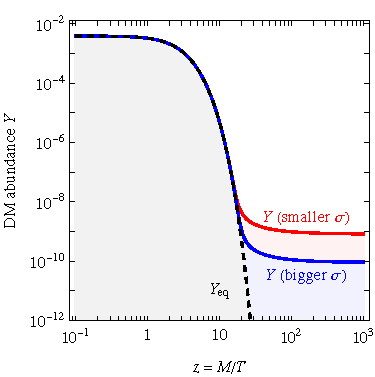
\includegraphics[width=0.45\textwidth]{figs/Ysample1}\qquad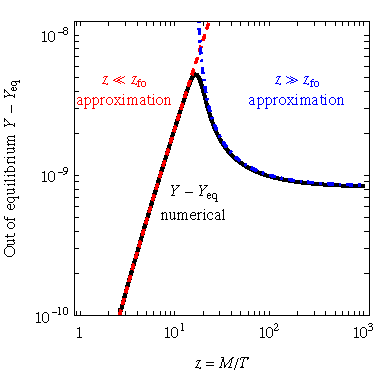
\includegraphics[width=0.45\textwidth]{figs/Ysample2}$$
\caption[Sample of DM freeze-out]{\em  \label{fig:Ysample} 
DM freeze-out examples.
{\bfseries Left}: sample of the evolution of the DM abundance $Y=n/s$ as function of $z=T/M$
for two different values of the DM annihilation cross section $\sigma$, compared to the equilibrium abundance $Y_{\rm eq}$ (dashed).
{\bfseries Right}: sample of the evolution of the non-equilibrium abundance
$Y-Y_{\rm eq}$, compared to the analytic approximations
in eq.\eq{beforefreezeout} (dashed, valid for $z\ll z_{\rm fo}$) and in
 eq.\eq{afterfreezeout} (dot-dashed, valid for $z\gg z_{\rm fo}$). 
}
\end{figure}

\index{s-wave annihilation} \index{p-wave annihilation}
Below we show instead how one can obtain precise analytic approximations, which are then compared with the numerical solutions in fig.\fig{Omegafreeze-out}b.
We assume that DM annihilates into lighter particles, so that this process is allowed also at very low temperatures.  
  In the non-relativistic limit, the expression for the annihilation rate  simplifies to
\beq
\label{eq:gamma:ann}
2\gamma_{\rm ann} \stackrel{T\ll M}{\simeq} {n_{\rm eq}^2} \langle \sigma v_{\rm rel} \rangle,
\eeq
where $ \langle \sigma v_{\rm rel} \rangle$ is the thermal average of  $\sigma v_{\rm rel}$.
In the non-relativistic limit the annihilation cross section can be expanded in powers of $v_{\rm rel}\ll 1$
as  $ \sigma v_{\rm rel} \simeq \sigma_0 + v^2_{\rm rel} \sigma_1 + \cdots $.
The leading $\sigma_0$ term is known as ${\mb s}${\bf-wave} and the sub-leading  $v^2_{\rm rel} \sigma_1$ term as ${\mb p}${\bf-wave}.
The thermal average is
  \beq 
  \label{eq:sigmasp}
 \langle \sigma v_{\rm rel} \rangle = \sigma_0 + \frac{6T}{M}   \sigma_1 + \cdots .
 \eeq
The Boltzmann equation for the total DM abundance then simplifies to    
\beq 
 \frac{dY}{dz} = -f(z) (Y^2 - Y^2_{\rm eq}),\qquad
f(z)\equiv \frac{s\langle\sigma v_{\rm rel}\rangle}{H Zz}
\stackrel{Z=1}{\approx} \frac{\lambda}{z^2}\left(1+\frac{6\sigma_1}{z\sigma_0}\right),
\label{eq:Boltzf}\eeq
where $Y_{\rm eq}\equiv n_{\rm eq}/s \stackrel{z\gg 1}{\simeq} g_{\rm DM}45 z^{3/2}e^{-z}/g_{\rm s}2^{5/2}\pi^{7/2}$,
having used $n_{\rm eq}$ from eq.\eq{neq}.
The dimension-less constant $\lambda$ is
\beq
 \lambda = \left.\frac{s\langle\sigma v_{\rm rel}\rangle}{H}\right|_{T=M}
=
{M_{\rm Pl} M \langle\sigma v_{\rm rel}\rangle}\sqrt{\frac{\pi \, g_{\rm s}^2}{45 \, g_\rho}}   \gg 1.\eeq

The estimate $\left.Y \sim 1/f \right|_{T \sim M}$ of eq.\eq{nDMestimate} is recovered by neglecting the inverse-annihilation
contribution $Y_{\rm eq}^2$ and writing eq.\eq{Boltzf} as
$d\ln Y/dz\sim - f Y$.
Furthermore,
we can derive the following approximate solutions, plotted in fig.\fig{Ysample}:
\begin{itemize}
\item[$\lhd$] Long before freeze-out, i.e.,\ at early
$z\ll z_{\rm fo}$, $Y(z)$ follows $Y_{\rm eq}(z)$ closely, so that one can expand to the first order in their small difference: explicitly, one recasts eq.\eq{Boltzf} in 
terms of $Y-Y_{\rm eq}$, neglects the $(Y-Y_{\rm eq})^2$ higher order term,  as well as the $(Y-Y_{\rm eq})'$ term  (here $'$ denotes the derivative with respect to $z$). One then finds an approximate solution for $Y$:
\beq 
Y(z)  \stackrel{z\ll z_{\rm fo}}{\simeq} Y_{\rm eq}  - \frac{Y'_{{\rm eq}}}{2f Y_{\rm eq}} \stackrel{z\gg 1}{\approx}
Y_{\rm eq}+\frac{z^2}{2\lambda},
\label{eq:beforefreezeout}
\eeq
where the last relation follows from applying the derivative on $Y_{\rm eq}(z)$ and recalling that we are always in the regime $z \gg 1$.
Next, we identify the moment of freeze-out, $z_{\rm fo}$, at which $Y(z)$ ceases to track $Y_{\rm eq}$. We define this to be the moment when the discrepancy $Y-Y_{\rm eq}$, which is just $z^2/2\lambda$ according to eq.~(\ref{eq:beforefreezeout}), becomes equal to $Y_{\rm eq}$ itself.
This gives the equation
\beq
z_{\rm fo} = \ln \frac{2 e \,\lambda  Y_{\rm eq}(1) }{\sqrt{z_{\rm fo}}},
\eeq   
which can be iteratively solved starting from $z_{\rm fo} \approx \ln \lambda Y_{\rm eq}(1) \approx 1/25$ (here $Y_{\rm eq}(1)$ is just a convenient short-hand way of writing the numerical coefficients in $Y_{\rm eq}(z)$).

\item[$\rhd$] Long after freeze-out, i.e.,\ at late
$z\gg z_{\rm fo} \approx 25$,
we can neglect the $Y_{\rm eq}^2$ term in eq.\eq{Boltzf}, giving a differential equation, $dY/dz = -f Y^2$,  which can be easily solved,
\beq  \frac{1}{Y_\infty}- \frac{1}{Y(z)} \stackrel{z\gg z_{\rm fo}}{\simeq} \int_\infty^z f(z)\,dz
=\frac{\lambda}{z}\Big(1+\frac{3\sigma_1}{z\sigma_0}\Big).\label{eq:afterfreezeout}
\eeq
Since $Y(z_{\rm fo})\gg Y_\infty$ we have the approximate solution  
\beq Y_{\infty}
=  \frac{z_{\rm fo} \sqrt{45 g_\rho/\pi g_{\rm s}^2}}{M_{\rm Pl} M (\sigma_0+3\sigma_1/z_{\rm fo})}.\label{eq:Yoo}
\eeq
\end{itemize}
If after freeze-out nothing in the evolution of the Universe changes the entropy in the visible sector, $Y_\infty$ can be identified with the present
DM entropy density, $Y_{\rm DM 0}$.
Converting it into the DM mass density via eq.~\eqref{eq:OmegaDMY} 
we obtain the precise version of the result announced in eq.\eq{OmegaDMapprox},
\beq \label{eq:Omegasigma0}
 \frac{\Omega_{\rm DM} h^2 }{0.110} =
  \frac{Y_\infty M}{0.40\eV} =
 \frac{z_{\rm fo}}{25} \frac{2.18~10^{-26}{\rm cm}^3/{\rm s}}{\sigma_0 + 3\sigma_1/z_{\rm fo}}.\eeq


Fig.\fig{Omegafreeze-out}b shows the precise value of $\sigma v_{\rm rel}$
 that reproduces the central value of DM cosmological abundance as a function of DM mass and of the number of DM  degrees of freedom.
 The somewhat counterintuitive result is that in these equations the number of degrees of freedom in the DM system only enters
with weak logarithmic dependence implicit in $z_{\rm fo}$. 
Note that $z_{\rm fo}\approx 25$ also means that a thermal relic DM has to be heavier than $M \circa{>} 10\MeV$. Lighter DM would have been in thermal equilibrium with the SM at $T \sim \MeV$, and this  would have increased the Hubble rate enough to conflict with the successful SM big-bang-nucleosynthesis results.





\subsection{Sample cross sections and the unitarity limit on the DM mass}\label{unitarity}
The treatment above is generic and model independent. The final result, eq.~(\ref{eq:Omegasigma0}), shows that the annihilation cross section
$\sigma v_{\rm rel}$ is the crucial parameter that determines the DM relic abundance.
Here we provide sample computations of annihilation cross sections in generic models, in order to make contact with the particle physics model parameters (essentially, couplings and masses).

\medskip

We consider a DM particle in a representation $R$ of an unbroken generic gauge group $\mathcal{G}$.
The non-relativistic
$s$-wave tree-level annihilation cross section into massless vectors is given by
\beq \label{eq:sigmavgeneric}
\sigma_0  = \frac{2C_R(C_R-C_G/4)}{ g_{\rm DM}}
\frac{\pi\alpha^2}{M^2},
\eeq
where $\alpha=g^2/4\pi$ is the gauge coupling,
$C_R$ is the quadratic Casimir defined in terms of generators as $\delta_{ij} C_R =(T^aT^a)_{ij}$;
$g_{\rm DM}$ is the number of DM degrees of freedom,
equal to $d_R$ for a real scalar, $2d_R$ for a complex scalar or for a Majorana fermion,
$4d_R$ for a Dirac fermion.
Here $d_R$ is the dimension of the representation.
The values of $d_R$ and $C_R$ in the adjoint representation are denoted as $d_G$ and $C_G$.
For $\mathcal{G}=\SU(2)$ one has $d_G=3$, $C_R = (d_R^2-1)/4$ for a generic representation with dimension $d_R$.
For $\mathcal{G}=\SU(3)$ one has $d_G=8$,
$C_3=4/3$, $C_8=3$, $C_{10}=6$, $C_{27}=8$, etc.
For $\mathcal{G}=\SU(N)$ one has $d_G=N^2-1$, $C_N = (N^2-1)/2N$, $C_{d_G}=N$.

\medskip

More in general, a typical $s$-wave $2\to 2$ DM annihilation cross section can be estimated as
 $\langle \sigma v_{\rm rel}\rangle = \sigma_0 \approx g^4/4\pi M^2$ where $g$ is some unspecified dimension-less DM coupling,
 such as a gauge or Yukawa coupling.
 Inserting this estimate in eq.\eq{Omegasigma0} implies that the DM mass which reproduces the cosmological DM abundance, is given by
 $M\approx g^2\times 6.5 \TeV$.
The perturbativity upper bound $g^2 \circa{<}4\pi$ then implies an upper bound on the DM mass:
 \beq\label{eq:100TeV}
 \bbox{M \circa{<}100\TeV}.\eeq
This is known as the\index{Unitarity bound}\index{Bounds!unitarity} {\bf unitarity bound}~\cite{unitaritybound}.\footnote{The often quoted bound $M \circa{<}340\, \TeV$ corresponds to the looser requirement $\Omega_{\rm DM} h^2 <1$, as in the original study~\cite{unitaritybound}.}
Its rigorous version for the $s$-wave cross section is 
$\sigma v_{\rm rel} \le 4\pi /M^2 v$.
However, waves with higher $\ell$ give extra contributions, such that in general no rigorous upper bound exists:
\beq 
\label{eq:unitaritybound}
\sigma v _{\rm rel} \le  \frac{4\pi}{M^2 v_{\rm rel}}\sum_{\ell=0}^\infty (2\ell+1) =\infty.\eeq
Indeed, bound states and more general classical objects with size $R$ have large geometrical cross sections $\sigma \sim \pi R^2$
after summing partial waves up to $\ell\circa{<}Mv_{\rm rel} R$, which is the classical angular momentum.
Model-dependent computations that try to determine which $\ell$ contribute by computing
 tree-level scatterings do not achieve a higher precision than estimates, given that the tree-level approximation
fails precisely when $g^2\sim 4\pi$.
Long-range forces can saturate the unitarity bound, as discussed in section~\ref{Sommerfeld}.


\medskip

At the other end of the spectrum, a lower bound on DM mass can be derived from the requirement of reproducing the cosmological DM abundance via annihilations. 
Assuming a DM particle that annihilates via the SM weak interactions through an $s$-wave process, 
the annihilation cross section is estimated as $\sigma_0 \approx G_{\rm F}^2 M^2/2\pi$, where $G_{\rm F} = \sqrt{2}g_2^2/8M^2_W$ is the Fermi constant. Inserting this estimate in eq.\eq{Omegasigma0} implies 
$M \gtrsim 3 \GeV$ in order to avoid a too large freeze-out DM relic density (i.e.~in order to have $\Omega_{\rm DM}h^2 \lesssim 0.110$). 
This is known as the\index{Lee-Weinberg bound}\index{Bounds!Lee-Weinberg} {\bf Lee-Weinberg bound}~\cite{LeeWeinberg}. 
Of course, this bound does not apply if DM has a different annihilation cross section,
not due to the SM weak interactions.\footnote{
Historically, the Lee-Weinberg bound presented a conceptual barrier against considering thermally-produced DM lighter than a few GeV. 
At the time, the dominant paradigm was a DM, typically fermionic, which annihilates via SM weak interactions. This scenario was  
motivated by supersymmetry and naturalness considerations (see section \ref{SUSY}), and the Lee-Weinberg bound  applies to it directly.
 In the early 2000s, however,  it was realized that, if DM particles annihilate via other forces rather than the SM weak interactions, then the bound can be circumvented, allowing for lighter DM to still be thermally produced in the right amount without overclosing the Universe. 
\index{Sub-GeV DM}
This conceptual breakthrough initiated the theoretical explorations of {\bf sub-GeV DM}~\cite{sub-GeVDM}.  The models of sub-GeV DM typically feature a dark photon or other light dark force mediators (see section \ref{sec:VectorPortal} for further details, as well as section \ref{cannibalism} for production mechanisms specific to sub-GeV DM, 
sections \ref{sec:direct:electrons}, \ref{sec:phonons} and \ref{BoostedDM} for direct detection of sub-GeV DM, section \ref{sec:IDconstraintsSub-GeV} for indirect detection, and section \ref{sec:searches:beam:dumps} for accelerator searches).}
Together with the more general eq.~(\ref{eq:100TeV}), it does define, however, the ballpark mass range for WIMP DM. 


\setstretch{0.95}
\subsection{Sommerfeld and bound-state corrections}
\label{Sommerfeld}
\index{Sommerfeld corrections}
\index{Bound state}
\index{DM properties!bound state}
Non-relativistic cross-sections can receive large non-perturbative corrections, known as the Sommerfeld corrections.
These effects tend to grow at low velocities, enhancing DM annihilations, and are thus relevant for cosmology (thermal freeze-out) and
indirect detection (section~\ref{chapter:indirect}), since in both processes DM is non-relativistic. 
Furthermore, since in galaxies DM has a lower typical velocity than it had during the freeze-out, the annihilation cross section in indirect detection can be  
above the standard freeze-out value, eq.\eq{sigmavcosmo}.

\medskip 

A classical analogy can help understand the physics: 
the cross section for falling into the sun (radius $R$, mass $M_\odot$)
equals the geometric area $\pi R^2$ only
for a body with a velocity much larger than the escape velocity
$v_{\rm esc} = \sqrt{2GM_\odot/R}$.
At lower  velocities the gravitational attraction increases the cross section to
$\sigma =\pi R^2 (1+ v_{\rm esc}^2/v^2_{\rm rel})$, 
where $v_{\rm rel}$ is the initial velocity of an infalling body (see also below).
A repulsive interaction would instead make the cross section smaller.

In the quantum regime, the non-relativistic cross sections for $e e$ scattering and $e \bar{e}$ annihilation
get distorted by the long-range electromagnetic interaction
when $v_{\rm rel} \circa{<} e^2$, i.e., in the regime where
the kinetic energy $\sim m_e v^2_{\rm rel}$ is smaller than the potential energy $e^2/r$ for separations
 comparable to the de Broglie wave-length, $r\sim 1/m_e v_{\rm rel}$.

\medskip

While DM has no electric charge and gravity is irrelevant at sub-Planckian energies,  
the Sommerfeld corrections can affect the non-relativistic DM annihilations~\cite{Sommerfeld}, if DM couples with dimension-less coupling $g$ to
a mediator particle with small mass, $M_V \ll M$. Such a light particle mediates what is effectively a long-range force relevant both in cosmology and in indirect detection. 
Such particle could be an electroweak vector gauge boson, if $M$ is well above the electroweak scale, or a new speculative `dark' vector coupled to DM, or a scalar
with a Yukawa (trilinear) coupling to fermionic (scalar) DM.


The Sommerfeld correction factor $S$, defined through $\sigma = S \sigma_{\rm pert}$ where $\sigma_{\rm per}$ is the perturbative (most often tree-level) cross section,
can be computed from the distortion of the wave function $\psi(\vec r)$
of the two-body DM-DM (or DM-$\overline{\rm DM}$)  initial state relative to the plane wave. To simplify the discussion let us focus on $s$-wave annihilation, and assume, at first, a massless mediator, giving a Coulomb like potential $V=-\alpha/r$ between the two DM particles.
Defining $\psi(\vec r) = u(r)/\sqrt{4\pi} r$, the function $u(r)$ satisfies  the  Schr\" odinger equation
$- u''/M - \alpha u/4\pi r  = E u$, with the outgoing boundary condition $u'(\infty)/u(\infty) \simeq iM v_{\rm rel}/2$.\footnote{The Sommerfeld correction could also be computed using incoming boundary conditions.}
The Sommerfeld factor  is then given by
$S = |u(\infty)/u(0)|^2$, and is
\beq  \label{eq:S0}
S = \frac{2\pi \alpha/v_{\rm rel}}{1-e^{-2\pi \alpha/v_{\rm rel}}}.\eeq
In the attractive case (corresponding to $\alpha >0$) $S$ grows for $ v_{\rm rel}\to 0$  roughly as $ S\propto v_{\rm max}/ v_{\rm rel}$ for  $ v_{\rm rel} <v_{\rm max} =\pi\alpha$. Note that this growth is still
consistent with the unitarity bound in eq.\eq{unitaritybound}.

If the mediator has mass $M_V$,
an analytic solution for $S$ can still be obtained by approximating the Yukawa potential 
with the Hulthen potential
\beq\label{eq:Hulthen}
 \frac{e^{- M_V r}}{r}\approx  \frac{  \kappa\, M_V e^{- \kappa M_V r }}{1- e^{-\kappa\, M_V r}},
\eeq
where the approximation is most accurate for $\kappa \approx 1.74$.
The  Sommerfeld factor is then
\beq\label{eq:Som}
S = \frac{2 \pi  \alpha  \sinh \left(\sfrac{\pi  M  v_{\text{rel}}}{\kappa 
   M_V}\right)}{v_{\text{rel}} \left[\cosh \left(\sfrac{\pi  M
   v_{\text{rel}}}{\kappa  M_V}\right)-\cosh \left(\sfrac{\pi  M
   v_{\text{rel}} \sqrt{1-\sfrac{4 \alpha  \kappa  M_V}{M
   v_{\text{rel}}^2}}}{\kappa  M_V}\right)\right]},
\eeq
and depends only on $\alpha/v_{\rm rel}$ and  $ \kappa M_V/M\alpha $.
In the case of an attractive potential, $S$  grows roughly as $ v_{\rm max}/ v_{\rm rel}$ in the range  
$M_V/M = v_{\rm min} < v_{\rm rel} <v_{\rm max} =\pi\alpha$,
and is constant at smaller $v_{\rm rel}$.
The Sommerfeld enhancement is therefore significant for $M_V < |\alpha| M$, and at temperatures
$T \circa{<}\alpha^2 M$.
Furthermore,  $S$ is resonantly enhanced when $M = \kappa n^2 M_V/\alpha$ for integer $n$,
which corresponds to a zero-energy bound state
(its decay width mitigates the resonant enhancement, see Blum et al.~in~\cite{Sommerfeld}).\footnote{If the long-range force is a non-abelian gauge interaction with vectors $V^a$, the potential
between particles in representations with generators $T_R$ and $T_{R'}$
becomes a matrix in component space.
As long as the group is unbroken,
its algebra allows to decompose the processes into effectively abelian sub-sectors,
$R\otimes R'= \sum_J J$, as
\begin{equation}
V= \alpha  \frac{ e^{-M_V r}}{r} \sum_a T_R^a\otimes  T_{R'}^a=\alpha \frac {e^{-M_V r}}{2 r} \left[\sum_J C_J  \One_J- C_R  \One_R - C_{R} \One_{R'}\right],
\end{equation}
where $C$ are the quadratic Casimirs
($C_n=(n^2-1)/4$ for DM in an $n$ dimensional representation of $\SU(2)$; $C_N =(N^2-1)/2N$ for DM in a fundamental ($N$-dimensional) representation  of $\SU(N)$, etc).
In each $J$ sub-sector  one gets an effective abelian-like potential 
\begin{equation}\label{eq:VQ}
V_J =-\alpha_{\rm eff}\frac {e^{-M_V r}}{r},\qquad \alpha_{\rm eff} = \frac{C_R+C_{R'}-C_J}{2} \alpha. \eeq}

\medskip

When Sommerfeld enhancements are relevant, a second related phenomenon is also important: the
formation of bound states of two Dark Matter particles with binding energy of order $\alpha^2 M$,
analogous to the  formation of hydrogen at recombination~\cite{BoundStates}.
Since the two DM particles within the bound state annihilate at a rate $\Gamma_{\rm ann}\sim \alpha^5 M$,
which is often cosmologically fast, the bound state effects can be described trough a modified
effective cross section, without writing a Boltzmann equation for each bound state,
see e.g.~\arxivref{1702.01141}{Mitridate et al.~(2017)} in~\cite{BoundStates}.

\medskip

Finally, these effects become more dramatic is DM is a bound state that forms at a QCD-like confinement scale $\Lambda$ that is much smaller than the DM mass $M$.\footnote{Composite DM will be further discussed in section \ref{sec:compositeDM}.}
Depending on the values of $M$, $\Lambda$ and of the consequent dark gauge coupling $\alpha$,
the cosmological cross section of eq.\eq{sigmavcosmo} needs to be equal either to
the perturbative cross section $\sim \alpha^2/M^2$ (if freeze-out occurs at $T \circa{<} M$),
or to the non-perturbative cross section $\sim 1/\Lambda^2$ (if non-perturbative bound states recouple later),
or to $1/M^2 \alpha^2$ (if perturbative bound states play a key role).
As a result the indirect-detection DM annihilation cross section predicted by cosmology can be 
$(M/\Lambda)^2$ larger than the standard value in eq.\eq{sigmavcosmo}.


\setstretch{1}
\subsection{$2\leftrightarrow 0$ co-annihilations}\label{sec:coann}
\index{Co-annihilations}\index{DM cosmological abundance!co-annihilations}
DM might be part of a `dark sector' that contains extra particles DM$'$ in addition to DM.
For example, in supersymmetric models DM can be the lightest supersymmetric particle;
in composite DM models the dark sector contains excited resonances.
Extra dark particles with masses $M'$ need to be taken into account in cosmological computations
of the relic abundance if $M' - M \circa{<}\hbox{few}\times T_{\rm dec}$ where $T_{\rm dec} \sim M/25$ is the 
decoupling temperature. The thermal abundance  of DM$'$ is suppressed relative to the DM one
by a Boltzmann factor $e^{(M-M')/T}$ so that for larger mass differences the abundance of DM$'$ becomes too small to be important, 
reverting  to the limit of a simple DM thermal freeze out discussed in section \ref{sec:reliccomputation}.

In the case of $N$ DM states with similar masses, $m_1\leq m_2\leq \cdots \leq m_N$,  the Boltzmann equation  for the number density $n_i$ for each of the particle species, $i=1,\ldots, N,$ is given by \cite{Griest:1990kh,Edsjo:1997bg}
\index{Boltzmann equation!for co-annihilations}
\beq
\begin{split}
\label{eq:coann:full}
\frac{dn_i}{dt}=&-3 H n_i-\sum_{j=1}^N\langle \sigma_{ij} v_{ij}\rangle \big(n_i n_j -n_i^{\rm eq} n_j^{\rm eq}\big)- \sum_{j\ne i}\Big[ \Gamma_{ij}(n_i -n_i^{\rm eq})-\Gamma_{ji} (n_j-n_j^{\rm eq})\Big]
\\
&- \sum_{j\ne i}\Big[\langle \sigma_{X ij} v_{iX}\rangle \big(n_i n_X-n_i^{\rm eq}n_X^{\rm eq}\big)-\langle \sigma_{X ji} v_{jX}\rangle \big(n_j n_X-n_j^{\rm eq}n_X^{\rm eq}\big).
\end{split}
\eeq
The first term on the r.h.s. gives the dilution of $n_i$ due to the expansion of the Universe. The second term describes the effects of the ${\rm DM}_i+ {\rm DM}_j$ {\em co-annihilations},  with the annihilation cross sections $\sigma_{ij} =\sum_X\sigma ({\rm DM}_i +{\rm DM}_j\to X)$, and the relative velocities in the thermal average given by $v_{ij}=\sqrt{(p_i\cdot p_j)^2- m_i^2 m_j^2}/E_i E_j$. Note that in this notation ${\rm DM}_1$ is the stable DM particle. The third term in eq.~\eqref{eq:coann:full} gives the contributions from the ${\rm DM}_i$ decays, with decay widths given by $\Gamma_{ij}=\sum_X \Gamma({\rm DM}_i\to {\rm DM}_j +X)$. The terms in the second line of \eqref{eq:coann:full} describe the ${\rm DM}_i\to {\rm DM}_j$ conversions on the SM thermal background (or on any other additional particles in the cosmic thermal plasma), with cross sections $\sigma_{Xij}=\sum_{X'}\sigma({\rm DM}_i+X\to {\rm DM}_j +X')$.

While the coupled Boltzmann equations for $n_i$ in eq.~\eqref{eq:coann:full} can be complicated, the problem simplifies significantly if we are only interested in the relic abundance of DM. The relic number density of DM is given by $n=\sum_i n_i$, as long as all the other states eventually decay to DM (plus SM states). (If this is not the case we are in a regime of {\em multi-component DM}.)  
The Boltzmann equation governing the time evolution of $n$ is much simpler, 
\beq
\frac{dn}{dt}=-3 H n-\sum_{i,j=1}^N\langle \sigma_{ij} v_{ij}\rangle \big(n_i n_j -n_i^{\rm eq} n_j^{\rm eq}\big),
\eeq
since in the sum the third and the fourth terms in eq.~\eqref{eq:coann:full} separately cancel. That is, for the total number of DM particles the conversions ${\rm DM}_i\leftrightarrow {\rm DM}_j$ do not matter because they conserve the total DM number.  

Further simplification is possible since the background number densities $n_X$ are much larger than the already Boltzmann suppressed DM number densities $n_i$, while the annihilations cross sections $\sigma_{ij}$ and $\sigma_{iX}, \sigma_{j,X}$ are usually comparable. This means that the last term in eq.~\eqref{eq:coann:full} ensures that ${\rm DM}_i$ remain in thermal equilibrium, and in particular $n_i/n\simeq n_i^{\rm eq} /n_{\rm eq}$. This then gives
\beq
\frac{dn}{dt}=-3 H n-\sum_{i,j=1}^N\langle \sigma_{\rm eff} v\rangle \big(n^2-n_{\rm eq}^2\big),
\eeq
where the effective annihilation cross section is given by 
\beq
\langle \sigma_{\rm eff} v\rangle=\sum_{ij}\langle \sigma_{ij} v_{ij}\rangle \frac{n_i^{\rm eq}}{n_{\rm eq}}\frac{n_j^{\rm eq}}{n_{\rm eq}}.
\eeq

From the expression for $\langle \sigma_{\rm eff} v\rangle$ we see that in the case where there are large mass splittings between ${\rm DM}_i$ and ${\rm DM}_1$, the contributions from ${\rm DM}_i$ are exponentially suppressed due to the Boltzmann suppressions, $n_i^{\rm eq}\ll n_1^{\rm eq}$ and thus $n_{\rm eq}\simeq n_1^{\rm eq}$. In this limit we recover the expression for the single DM thermal freeze out. For $m_i\simeq m_1$, on the other hand, all the ${\rm DM}_i$ contribute to the effective annihilation cross section. In particular, the ${\rm DM}_1 +{\rm DM}_1$ annihilation can be heavily suppressed, and nevertheless  $\langle \sigma_{\rm eff} v\rangle$ can be large due to the contributions from ${\rm DM}_i$, $i\ne 1$.  This is the case, for instance, when ${\rm DM}_i$ carry color charges and thus have large annihilation cross sections controlled by QCD, typically much larger than the ${\rm DM}_1+ {\rm DM}_1$ annihilation cross section. Without such additional annihilations the ${\rm DM}_1$ would have had a much larger relic abundance $\Omega_{\rm DM}\propto 1/\langle \sigma_{11} v_{11}\rangle$. However, due to the presence of extra  ${\rm DM}_i$ states the excess ${\rm DM}_1$ convert to ${\rm DM}_i$ through scatterings on the SM background, and then the ${\rm DM}_i$ annihilate away, resulting in a smaller relic abundance  than if ${\rm DM}_i$ were not present (that is, in this case $\langle \sigma_{\rm eff} v\rangle$ is larger than $\langle \sigma_{11} v_{11}\rangle$). 

The converse can also be true. If $ \sigma_{ij}\ll  \sigma_{11}$, it is possible that $\langle \sigma_{\rm eff} v\rangle$ is smaller than $\langle \sigma_{11} v_{11}\rangle$. In this situation ${\rm DM}_1$ annihilates away through  ${\rm DM}_1+{\rm DM}_1$ process, but is being repopulated through ${\rm DM}_i\to {\rm DM}_1$ conversions on the cosmic thermal plasma background. In this case the DM relic abundance is larger than if the extra ${\rm DM}_i$ states with small annihilation cross sections were not present. 


\subsection{$2\leftrightarrow 1$ semi-annihilations}
\index{Semi-annihilations}\index{DM cosmological abundance!semi-annihilations}
Recalling that we count only the number of DM-sector particles, so that 
any number of SM particles can be present,
the $2\leftrightarrow 1$ notation  means that we now allow for extra processes such as
\beq {\rm DM}_i {\rm DM}_j\leftrightarrow {\rm DM}_k {\rm SM},\eeq 
where SM is one or more particles in the SM sector.
These processes, known as {\em semi-annihilation}~\cite{semiann}, would add
an extra term $-\gamma_{2\leftrightarrow 1}   (\sfrac{Y^2}{Y^{2}_{\rm eq}}-\sfrac{Y}{Y_{\rm eq}})$
on the r.h.s.~of the Boltzmann equation\eq{DMboltzY}.
Their effect is similar to annihilations.
Semi-annihilations arise in models where DM particles are stable because of a symmetry 
different than a $\mathbb{Z}_2$ reflection, ${\rm DM}\to - {\rm DM}$.
A concrete example is DM whose constituents are the  massive vectors $Z', W'$ of a dark
$\SU(2)'$ gauge group, broken by a dark scalar doublet $H'$ that mixes with the Higgs doublet $H$~\cite{semiann}.
Cubic gauge interactions among dark vectors lead to semi-annihilations.
Such DM is stable for the same reason that the SM gauge bosons $Z,W$ would have been stable, had the SM fermions not been present.

\smallskip

In these kinds of models all the DM states can be stable, if the decay processes ${\rm DM}_k \to {\rm DM}_i {\rm DM}_j {\rm SM}$ are kinematically forbidden.
For example, in the SM without electroweak interactions the proton $p$, the neutron $n$, and the charged pions $\pi^\pm$ would all be stable, despite the presence of semi-annihilations such as $p\pi^-\to n \pi^0$ 
(where $\pi^0$ would decay into $\gamma\gamma$ as usual).

Note that, if DM initially only has a small abundance, it is increased exponentially by the inverse semi-annihilations, the $1\to 2$ scatterings~\cite{semiann}.

The $2\leftrightarrow 1$ processes of the form ${\rm DM}_i {\rm DM}_j {\rm SM} \leftrightarrow {\rm DM}_k {\rm SM}$, which have in the initial state an extra SM particle with low abundance (such as relic protons with well below thermal abundance, $n_p\ll n_\gamma$),
 behave similarly to the $3\leftrightarrow 2$ processes 
to be discussed in section~\ref{sec:3<->2eq}~\cite{CoSIMP}.



\subsection{$1\leftrightarrow 0$ thermal decays}
The notation $1\leftrightarrow 0$ means that we now consider processes where one DM particle
disappears, and any number of SM particles can be present.
So, for example, we here study  DM undergoing processes of the type
\beq {\rm DM}\,  {\rm SM} \leftrightarrow {\rm SM}\, {\rm SM}.\eeq
These processes, dubbed {\em thermal decays}, would add an extra term
$ -\gamma_{1\leftrightarrow 0}   (\sfrac{Y}{Y_{\rm eq}}-1)$
 on the r.h.s.~of the Boltzmann equation\eq{DMboltzY}. 
If DM scatters on a light SM particle, thermal decays are
more efficient than annihilations, because they are less Boltzmann suppressed at temperatures $T \circa{<}M$. Consequently, 
the  final DM abundance  can be suppressed by a smaller power of the cross section
than in the case where the DM abundance is set purely by annihilations, eq.\eq{afterfreezeout}.

\smallskip

Thermal decays are only present in theories where there is no $\mathbb{Z}_2$ or any other symmetry that would
separate the dark sector from the SM sector, and prevent DM from decaying.
In these theories DM therefore undergoes decays also at zero temperature, which is phenomenologically challenging given that DM decays are
subject to very strong bounds, as discussed in section~\ref{chapter:indirect}.
The DM decay width must be roughly 30 orders of magnitude smaller than
the finite-temperature DM decay rate needed to achieve thermal equilibrium at $T\sim M$,
 $\gamma_{1\leftrightarrow 0} \approx n_{\rm DM} \Gamma_{{\rm DM}T}$ with $\Gamma_{{\rm DM}T}\sim H$.
Consequently, the relic DM abundance is set through thermal decays 
only in very special theories~\cite{Thermaldecays}.

\subsection{$3\leftrightarrow 2$ DM processes in a decoupled dark sector}\label{cannibalism}
\label{DM cosmological abundance!cannibalism}
The notation $3\leftrightarrow 2$ means that we now consider processes
where DM-sector particles undergo processes such as
\beq \hbox{DM DM DM} \leftrightarrow \hbox{DM DM}\eeq
and any number of extra SM particles could be present on both sides.
These processes occur when DM has significant self-interactions
 that lead to number-changing scatterings,
 for example, through a combination of cubic and quartic interactions of scalar DM.
Even though the DM number is no longer conserved,
DM can still be stable on cosmological timescales, if in the dark sector there are no other particles lighter than the DM,
and the interactions with light SM particles are small enough.
An example of a concrete UV model that leads to $3\leftrightarrow 2$ scattering is DM that is a glue-ball of a new confining non-abelian gauge interaction in the dark sector.

\medskip

Let us first focus on the simplest case; that of a completely decoupled dark sector~\cite{cannibalism}, without any interactions with the SM. As we will see below, in this case the $3\leftrightarrow 2$ scatterings do not provide a viable mechanism for DM production. This is quite different from the other DM production mechanisms that we studied so far, all of which would have worked also if only the (appropriate) dark sector were involved. 

The challenge for the decoupled dark sectors with $3\leftrightarrow 2$ scatterings is that when the temperature $T_{\rm DM}$ in the dark sector becomes smaller than $M$,
the scatterings such as DM DM DM $\to$ DM DM heat the dark sector, keeping it at $T_{\rm DM}\sim M$.
This was dubbed `{\bf cannibalism}'~\cite{cannibalism}, because the heating occurs at the price of the DM number:
DM keeps warm by eating itself.
Cannibalism ends at the decoupling temperature $T_{\rm DM}^{\rm dec}$, at which point 
DM gets so diluted that the cannibalistic scatterings become slower than the rate of the expansion of the Universe, and drop out of thermal equilibrium.
The predictions for the cannibalistic phase are easy to compute since the comoving entropy $s a^3$  is conserved separately in each of the two decoupled sectors: SM and DM.
In the SM sector this gives the usual $T_{\rm SM}\propto 1/a$.
In the DM sector one has $s_{\rm DM}\equiv (\rho_{\rm DM}+p_{\rm DM})/T_{\rm DM}  \approx M n_{\rm DM}^{\rm eq}/T_{\rm DM}$,
where the non-relativistic number density $n_{\rm DM}^{\rm eq}$ of eq.\eq{nnonrel}
contains the exponential factor $e^{-M/T_{\rm DM}}$.
In view of this factor, during cannibalism $T_{\rm DM}$ decreases only logarithmically,
$T_{\rm DM} \simeq M/3\ln(a/a_M)$, where $a_M$ is the scale factor at which $T_{\rm DM}=M$.
The possibility that the cannibalistic phase happens during matter domination is subject to constraints,
because a cannibalistic dark sector affects large scale structures differently from ordinary dark matter~\cite{cannibalism}.
After decoupling, the dark sector no longer self-interacts, and starts behaving as ordinary dark matter: 
$\rho_{\rm DM}$ and $s_{\rm DM}$ scale as $1/a^3$.
The conserved ratio $\xi \equiv s_{\rm SM}/s_{\rm DM}$ is of order one if the SM and DM
sectors have been initially in equilibrium at $T \gg M$.
The predicted DM abundance is therefore
\beq Y_{\rm DM}\equiv \frac{n_{\rm DM}}{s} \approx \frac{s_{\rm DM} T_{\rm DM}^{\rm dec}/M}{s_{\rm SM}}.\eeq
The cosmological DM abundance is reproduced for $Y_{\rm DM} \approx 0.4\eV/M$, see eq.\eq{YDM0}.
The DM decoupling temperature is thereby
\beq 
T_{\rm DM}^{\rm dec}\approx 0.4\eV\, \xi,
\eeq
independently of the DM model.
Unless $\xi$ is very large, this is problematic in two ways: 
such low $T_{\rm DM}^{\rm dec}$ would affect standard cosmology and for instance lead to problems with BBN. 
It also implies that the DM mass is not much above the eV scale, with too large DM self-interactions.
Very large $\xi$ can be obtained if the dark sector is populated through freeze-in.

\medskip

While the simplest version of cannibalism is excluded as the DM production mechanism, more complicated variants of this scenario are allowed.
For example, some heavier unstable dark sector particle DM$'$ could
undergo `cannibalistic' $2\leftrightarrow 3$ scatterings, 
where the cooling of SM plasma temperature, $T_{\rm SM}$, compared to dark sector one, $T_{\rm DM}$, is interrupted when DM$'$ decays~\cite{cannibalism}.
Alternatively, DM could remain kinetically coupled to the SM during (part of) the cannibalistic phase, 
so that the SM sector is reheated possibly up to the dark sector temperature~\cite{cannibalism,MeVDM}.
This possibility is studied in the next section.

\subsection{$3\leftrightarrow N$ and $4\leftrightarrow N$ in thermal equilibrium}\label{sec:3<->2eq}
As in the previous section, we assume that DM undergoes processes such as 
DM DM DM $\leftrightarrow$ DM DM, denoted as $3\leftrightarrow 2$.
However, this time we also assume that some process keeps DM in thermal equilibrium with the SM sector, 
so that the two have a common temperature~\cite{MeVDM}.
The thermalising interaction can also give DM DM $\leftrightarrow$ SM SM scatterings: 
we assume that their effect can be neglected
in the Boltzmann equation for the DM abundance $Y$ \index{Boltzmann equation!for $2\leftrightarrow 3$}
\beq sHZz\, 
 \frac{dY}{dz} =  \gamma_{3\leftrightarrow 2}  \left(\frac{Y^2}{Y^{2}_{\rm eq}}-\frac{Y^3}{Y^{3}_{\rm eq}}\right).\eeq
This can be compared with the Boltzmann equation  in eq.\eq{DMboltzY} for $2\leftrightarrow 0$ annihilations.
The quick estimate of the DM relic abundance for $2\to 0$ process, presented in section~\ref{sec:thermalapprox}, can be 
adapted to the $3\leftrightarrow 2$ case, as follows.
DM freezes-out at $T=T_{\rm dec}$, when the DM interaction rate is comparable to the Hubble rate $\Gamma_{3\leftrightarrow 2} \sim H$.
The interaction rate $\Gamma_{2\leftrightarrow0}=\langle \Phi \sigma_{2\leftrightarrow0} \rangle$ 
gets replaced by $\Gamma_{3\leftrightarrow 2} \approx  \langle \Phi^2\sigma_{3\leftrightarrow2}\rangle$.
Here $\Phi =n_{\rm DM} v$ is the DM flux, and dimensional analysis fixes 
the $3\to2$ analog of the $2\to 0$ cross section $\sigma_{2\leftrightarrow0}$
to have the form $\sigma_{3\leftrightarrow2} \sim \alpha^3/ M^5$,
where $g$ is some DM self-coupling and $\alpha=g^2/4\pi$.
Omitting order one factors, we have $T_{\rm dec}\sim M$ and $v\sim 1$, and the relic DM density
is 
\beq
Y\sim \frac{1}{M^2\sqrt{M_{\rm Pl} \sigma_{3\leftrightarrow2}}}\sim \sqrt{\frac{M}{M_{\rm Pl}\alpha^3}}.
\eeq
Note that $Y$ is 
suppressed by a smaller power of $M_{\rm Pl}$ than in the $2\leftrightarrow0$ case.
As a result the observed DM cosmological abundance, $Y \sim \eV/M$,
is matched for  lighter DM
\beq \label{eq:3<->2estimate}
M/\alpha \sim (\eV^2 M_{\rm Pl})^{3/2}  \sim \GeV.\eeq
In addition to $3\leftrightarrow2$ DM processes, specific models
can predict $2\leftrightarrow2$  scatterings among DM, with cross section
$\sigma/M \sim \alpha^2/M^3$. This are potentially large enough that they risk conflicting with the bullet cluster bound in eq.\eq{bulletbound},
unless $M$ is as heavy as possible. Eq. \eqref{eq:3<->2estimate} then implies large $\alpha$.



 \smallskip
 
So far  we assumed full thermal equilibrium between DM and the SM, 
while the opposite was assumed in section~\ref{cannibalism}.
An intermediate regime, where thermalization interactions decouple, while the
$3\leftrightarrow 2$ scatterings are still active, is also possible, see~\cite{MeVDM} for further details.

\smallskip

The DM models with $3\leftrightarrow2$ scatterings that received quite some attention 
have dark pions as DM states, with some SM interactions (see section~\ref{sec:darkpi}). Another possibility discussed in the literature is 
quartics among dark scalars, imposing $\mathbb{Z}_3$ or $\mathbb{Z}_5$
symmetries. These could possibly be remnants of a dark U(1) gauge symmetry broken by a scalar with charges 3 or 5~\cite{MeVDM}.

\smallskip

Note that having 2 DM particles in the final state played no role in the estimate in eq.\eq{3<->2estimate}.
Therefore the same estimate, up to order unity factors, also applies to the case of pure $3 \leftrightarrow0$ or $3 \leftrightarrow1$ processes
(we recall that our notation counts the number of dark sector particles, allowing for any number of extra SM particles).
Possible models for such processes can be obtained considering dark scalars with quartic couplings, such as $SSSS'$.
However, these $3 \leftrightarrow 0,1$ processes have little interest because they are accompanied by 
more efficient  $2 \leftrightarrow 1,2$ scatterings,
obtained by moving one dark sector particle from the initial to the final state
(these related processes can be suppressed in special models with a large asymmetry in the dark sector).

\medskip

Finally, we consider scatterings among more the 3 dark-sector particles.
The estimate in eq.\eq{3<->2estimate} can be extended to the case of $4\leftrightarrow2$ DM annihilations:
the corresponding rate is given by
$\Gamma_{4\leftrightarrow2} \sim \Phi^3 \sigma_{4\leftrightarrow2} $ with
$\sigma_{4\leftrightarrow2} \sim \alpha^4/M^8$, leading
 to the estimate $M/\alpha \sim (\eV^3 M_{\rm Pl})^{1/4}\circa{<}\MeV$ for the DM mass. 
 This is typically excluded.

\subsection{Special freeze-out kinematical configurations}
Specific limits of the thermal freeze-out mechanism can lead to significant deviations from the generic estimates discussed above, with phenomenological implications. 
Examples include the following.
\begin{enumerate}
\item The `{\bf forbidden DM}' limit occurs when DM is lighter than any of the SM states it can annihilate into \cite{Forbidden:DM}. 
This means that $\text{DM}\,\text{DM}\to \text{SM}\,\text{SM}$ annihilation is kinematically open for $T \gg M$, 
while at the freeze-out temperatures only the DM particles on the higher-energy tail of the thermal distribution can annihilate. 
This scenario can be realized, if DM has negligible couplings to the SM particles that are lighter than DM (such as photons and neutrinos).
`Forbidden DM' evades CMB bounds on light DM, because DM annihilations are highly suppressed at the low temperatures relevant for the CMB. 
The CMB bounds are evaded even if the splittings between DM and the states it annihilates to are tiny (this scenario was termed the `{\bf impeded DM}'~\cite{1609.02147}). 

\item DM DM annihilations can be mediated by a resonance in the $s$-channel and be {\bf near the pole} for specific DM energies. 
This was discussed in section \ref{Sommerfeld}.

\item {\bf Decoupling of inelastic scattering} (or the so called {\bf co-scattering}) occurs when $\text{DM}\,\text{DM}$ annihilations are negligible, while 
the DM cosmological abundance decreases through inelastic scatterings, 
$\text{DM}\,\text{SM}\to \text{DM}'\, \text{SM}$, followed by ${\rm DM}'\,{\rm DM}'$ annihilations~\cite{1705.08450}. 
The required scattering cross section is very different from the simple thermal freeze-out; 
in particular, the DM mass is generically much lighter than the weak scale. 
Furthermore, the $\text{DM}\,\text{DM}$ annihilation rate can be arbitrarily small, thus avoiding CMB constraints on light DM. 

\item {\bf Co-annihilation of split states.} Usually, co-annihilation of DM is important when there are dark states with masses similar to the DM particle.
However, if the DM self-annihilation is suppressed, co-annihilations with states in the dark sector significantly heavier than DM
become relevant for setting the DM relic abundance. 
This limit can lead to the correct relic abundance even for very light DM, down to the keV scale~\cite{1803.02901} (see also section \ref{sec:coann}). 
\end{enumerate}

\subsection{Special freeze-out cosmological configurations}
So far we assumed standard cosmology while DM freezes out, at $T \sim M/25$.
This needs not be the case, since the DM freeze out likely occurred before the Big Bang Nucleosynthesis, at temperature well above $T \gtrsim \MeV$ and cosmology is largely untested at such high temperatures.
A non-standard cosmological history can result in significant deviations from the generic estimates discussed above, with essentially endless variations still possible. 
Concrete examples include:
\begin{enumerate}
\item If the Universe underwent a phase of fast expansion, this affected the DM relic abundance~\cite{relentless}. 
For example, if the Universe contains an exotic fluid whose energy density evolved as 
$\rho \propto a^{-3(1+w)}$ with $w>1/3$, and thus redshifted faster than radiation (see eq.\eq{p=wrho}), 
this fluid dominated the energy budget of the Universe at very early times, before the era of radiation domination. 
This induced a phase of fast expansion. 
A concrete realization discussed in the literature is the so called {\bf `kination'} phase, 
in which the energy budget of the Universe is dominated by the kinetic energy of a time-dependent scalar field. 
This could be the quintessence field, which in the late stages of the evolution of the Universe gives rise to Dark Energy.
   
Since in this case the Universe during freeze-out expands faster than it does in the standard cosmology, 
the correct DM abundance is reproduced via freeze-out with a
DM annihilation cross section $\langle \sigma v \rangle$ {\em larger} than the standard one of eq.~(\ref{eq:sigmavcosmo}). 
Because of the larger annihilation cross-section, DM keeps annihilating  longer, after departing from thermal equilibrium. 
This scenario has thus also been termed `{\bf relentless DM'} \cite{relentless}. 


\item The Universe is believed to have gone through a phase of exponential inflationary expansion at very early times, see section \ref{sec:inflDMprod}. If the Universe has also undergone a later short period of fast expansion, sometimes called `late time inflation', then the density of any particle species 
(including DM) that had already decoupled by the beginning of the late time inflationary period would have been significantly {\bf diluted}~\cite{dilutionofDM}.
Once late-time inflation ends, its energy density reheats light SM particles while DM is too heavy.
In these models, DM needs an annihilation cross section $\langle \sigma v \rangle$ much {\em smaller} than what is needed 
for the standard thermal freeze-out, and that would have otherwise lead to an over-abundant DM in the standard cosmology.
The idea of inflationary dilution is simple and general and can be applied to other models featuring over-abundant DM, e.g., to axions with `too large' $f_a$ (see section \ref{AxionCosmo}). A specific realization of this setup is discussed in section \ref{supercoolingproduction}.

\item A different kind of dilution of the DM density occurs if, after DM freeze-out, 
the Universe underwent a phase of {\bf early matter domination}~\cite{DM:entropy:injection}. 
This happens if the energy budget of the Universe becomes temporarily dominated by metastable particles. 
If these are sufficiently heavy and their lifetimes long enough (but short enough to avoid conflicts with Big Bang Nucleosynthesis bounds), they may temporarily dominate the energy density of the Universe, so that, when they eventually decay, they {\bf inject significant entropy} in the SM bath and thus dilute any relic abundance, including that of DM \cite{DM:entropy:injection}. Assuming that the mass of the decaying particle is sufficiently small ($M^\prime <2M$), guarantees that its decays can not reheat DM itself. If the freeze-out had resulted in overabundant DM, even up to equilibrium-like abundances $n_{\rm DM} \sim n_\gamma$, the mechanism can then dilute it down to the observed density.

\end{enumerate}
The latter two possibilities allow for a smaller cross section at freeze-out time, and therefore for a {\em larger DM mass}, possibly above the unitarity limit (see section \ref{unitarity}). In concrete models these extra decaying particles can belong to the dark sector, or mediate interactions between the dark and the SM sectors (an example of such a mediator is a $Z'$ vector boson).
 
 

\section{DM as a non-thermal relic}\label{sec:freeze-in}
Freeze-out from thermal equilibrium is a generic mechanism that applies to any interacting massive
particle. One of its main attractive features is that in its simplest form it predicts the DM relic abundance just from annihilation cross section (with very small dependence on DM mass).
Many other, less predictive scenarios are also possible.
Below, we briefly summarize some of them.\footnote{For a systematic appraisal of DM production mechanisms, including freeze-out, freeze-in and others, see also \arxivref{1112.0493}{Chu et al.~(2012)}~\cite{1112.0493}.}

\subsection{Freeze-out and decay}\label{sec:freezeoutdecay} \index{Super WIMPs}
A rather straightforward extension is that the thermal relic is not the DM itself, but rather another particle $X$, which decays 
into DM after freeze-out~\cite{SuperWIMP}. This results in a DM density $\Omega_{\rm DM} = \Omega _X M/M_X$, up 
to extra model-dependent corrections, e.g.,\ if the decay is slow enough that the decays reheat the universe. 
Since $M_X>M$ the correct relic abundance is obtained for smaller annihilation cross sections than eq.~\eqref{eq:sigmavcosmo}. Gravitino DM (see section \ref{sec:gravitinoDM}) is a good example of a realization of this scenario. 



\begin{figure}[t]
$$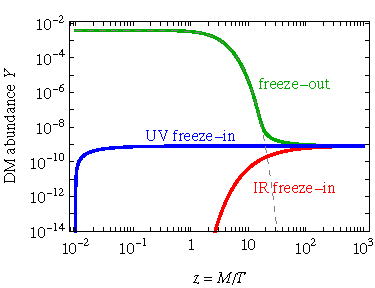
\includegraphics[width=0.45\textwidth]{figs/Ysampleinout}$$
\caption[Illustration of freeze-in and freeze-out DM abundance evolution]{\em\label{fig:Ysamplein} Illustration of the cosmological evolutions of DM 
abundance $Y=n/s$ for the IR (red curve) and the UV (blue) freeze-in, compared to the freeze-out (green),
and the thermal equilibrium abundance (dashed).
}
\end{figure}


\subsection{Freeze-in}\label{Freeze-in}
\index{Boltzmann equation!for freeze-in}
\index{Freeze-in}\index{DM cosmological abundance!freeze-in}
A possible explanation for the small cosmological density of DM, $Y_{\rm DM} \approx 0.4\eV/M  \ll 1$ for $M\gg \eV$, 
could be that 
DM is a particle that is so weakly coupled to the rest of the Universe
that its initial abundance was vanishingly small.
Small interactions of DM with the SM thermal bath then produced a sub-thermal DM abundance $Y_{\rm DM} \ll 1$,
given by
\beq \label{eq:FIestimate}
Y_\infty = \int_0^\infty \frac{dz}{z}   \frac{N \gamma}{H s}
\sim  \max_T \frac{N \gamma}{H s},
\eeq
where $\gamma$ is the space-time density of SM interactions that produce $N$ (usually 2) DM particles.
In this situation, the primordial DM velocity distribution would contain information about the production mechanism.
This can happen in two main qualitatively different ways, illustrated in fig.\fig{Ysamplein}:
\begin{itemize}
\item[$\blacktriangledown$]
{\bf IR freeze-in}.
DM particles which have {\em small renormalizable interactions} $g$ with the SM
are dominantly produced at the lowest possible
temperatures, typically at temperatures that are a factor of a few below their mass $M$~\cite{freeze-in}.\footnote{A variation is the `Leak-in DM' scenario~\cite{Evans:2019vxr}, in which the small interactions do not produce directly the DM particles but rather populate the hidden sector which subsequently thermalizes and therefore generates DM particles internally.}
The space-time density of scatterings that produce DM particles from the SM plasma is
roughly $\gamma \sim g^4 T^4$.
The resulting DM abundance is $Y_{\rm DM}  \approx \gamma/Hs|_{T\sim M} \sim g^4 M_{\rm Pl}/M$, 
which matches the cosmological DM density in eq.\eq{YDM0}
for $g \sim (Y_{{\rm DM}0} M/M_{\rm Pl})^{1/4}\sim (T_0/M_{\rm Pl})^{1/4}\sim 10^{-8}$.
For example, fig.\fig{chargedDM} shows that 
DM with a small electric charge needs $qe \approx 10^{-11}$ for any DM mass $M \circa{<}T_{\rm RH}$ 
(the reheating temperature $T_{\rm RH}$ is the largest temperature achieved in the evolution of the Universe and thus sets the upper bound on the mass of the heaviest particle that can be produced).
Since the freeze-in DM is predominantly produced in the mildly relativistic regime,
the precise computations depend on the details about DM  interactions:
the non-relativistic cross section $\sigma_0$  that we introduced when we were studying the freeze-out, see eq. \eqref{eq:sigmasp},
can only be used to obtain an indicative value,
$Y_{\rm DM} \approx g_{\rm SM} M M_{\rm Pl} \sigma_0/g_{\rm SM}^{3/2}$.
A precise computation is possible, if DM is dominantly produced via {\em decays} of a heavier
particle into $N$ DM particles (the heavy particle has mass $M'$, $g'$ degrees of freedom, and decay width $\Gamma'$).
The DM production rate is given by eq.\eq{gammaD}, resulting in
\beq \label{eq:decayfreezein}
Y_{\rm DM} =\int_0^\infty \frac{dz}{z}   \frac{\gamma^{\rm eq}_{\rm decay} }{H s}= 
\frac{405N\sqrt{5} M_{\rm Pl} g' \Gamma'}{16\pi^{9/2} g_{\rm SM}^{3/2} M^{\prime 2}}.\eeq
Unlike freeze-out, the IR freeze-in allows for DM to be lighter than an MeV, without conflicting with the big-bang nucleosynthesis constraints. 



\item[$\blacktriangle$] 
{\bf UV freeze-in}. 
DM particles which possess {\em small non-renormalizable interactions} with the SM particles 
are dominantly produced at the highest possible temperature $T_{\rm RH}$ 
and thereby their abundance depends on $T_{\rm RH}$.
Since the value of $T_{\rm RH}$ is unknown, there are no  unambiguous predictions.
The reheating temperature after inflation with Hubble constant $H_{\rm infl}$ is $T_{\rm RH} \sim \sqrt{M_{\rm Pl} H_{\rm infl}}$, if the inflaton $\phi$ decays promptly, and is lower otherwise, given by
$T_{\rm RH}\sim \sqrt{M_{\rm Pl} \Gamma_\phi }$, where $\Gamma_\phi$ is the decay width of the inflaton. 
Indeed, in the latter case, the entropy release from inflaton decay ends when $\Gamma_\phi \sim H \sim \sqrt{\rho_\phi}/M_{\rm Pl}$ giving $T_{\rm RH}^4\sim \rho_\phi$.
UV freeze-in can work with larger couplings if the DM mass is mildly above $T_{\rm RH}$.
If the non-renormalizable operators are mediated by renormalizable interactions of particles lighter than $T_{\rm RH}$,
then one reverts back to the IR freeze-in: 
the DM particles are predominantly produced at temperatures close to the mass of the mediator.





\end{itemize}
Gravity is one known non-renormalizable interaction, roughly corresponding to $g \sim T/M_{\rm Pl}$.
Gravitational DM production can be estimated as follows:
\begin{itemize}
\item[$-$]
Purely gravitational scatterings give $\gamma \sim T^8 e^{-2M/T} /M_{\rm Pl}^4$
resulting in $Y_{\rm DM}  \approx \gamma/H s|_{T =T_{\rm RH}}  \sim (T_{\rm RH}/M_{\rm Pl})^3 e^{-2M/T_{\rm RH}}$.
DM particles with only gravitational interactions are discussed in section~\ref{GravDM}.
\item[$-$]
A special case is the gravitino (see section~\ref{sec:gravitinoDM}), 
a spin 3/2 fermion motivated by supersymmetry,
whose dominant interactions to the SM, such as the coupling to gluons and gluinos, can be of gravitational strength.
Gravitinos can then be produced in processes that combine QCD with gravitational interactions, resulting in
$\gamma \sim g_{\rm s}^2 T^6 e^{-M/T} /M_{\rm Pl}^2$.
Inserting $g_{\rm s} \sim 1$ and
assuming $M \ll T_{\rm RH}$ (such that the gravitino is long-lived),
the gravitino number abundance is
$Y_{\rm DM}  \approx \gamma/H s|_{T =T_{\rm RH}}  \sim T_{\rm RH}/M_{\rm Pl}$, corresponding to
$\Omega _{\rm DM} \sim (M/\TeV)(T_{\rm RH}/10^{10}\GeV)$~\cite{gravitinoCosmo}.
Another example is KK gravitons, that will be discussed in section~\ref{sec:swampDM}.
\end{itemize}
It is worth mentioning that the dominant DM interaction being
 $1\to N$ decay with rate $\Gamma$, 
rather than a $2\leftrightarrow 2$ scattering, is phenomenologically not viable.
The decays would give a freeze-in abundance $Y_{\rm DM} \sim \Gamma/H$ at $T \sim M$, so $Y_{\rm DM} \sim M_{\rm Pl} \Gamma/M^2$.
The resulting DM abundance $\Omega_{\rm DM} \sim M_{\rm Pl} \Gamma/M  \eV$
is negligible, $\Omega_{\rm DM}  \sim 10^{-8}$, even in the most favorable case:
$M \sim\,{\rm keV}$ and $\Gamma \sim 1/(10^{10}\,{\rm yr})$. Experimental bounds on realistic models (see e.g.~\ref{FermionSinglet})
give much stronger constraints on $\Gamma$.

\medskip

Before accepting freeze-in as a viable possibility, one must consider whether this mechanism generates DM inhomogeneities
compatible with observations. Importantly, perturbations
on (current) cosmological scales need to be adiabatic rather than iso-curvature.
Adiabatic means that there is a unique fluid with the same SM/DM relative density everywhere,
while iso-curvature means that there are entropy fluctuations in the relative density.
In the case of freeze-out, adiabaticity is enforced by thermal equilibrium~\cite{AdiabaticDM}.
In the case of freeze-in, adiabaticity holds on scales larger than the (small) horizon at freeze-in,
because different regions of the universe can be seen as `separated universes' that undergo the same freeze-in
dynamics up to the time delay $\delta t(t,\vec{x})$. Since the time delay is common to all components in a particular patch of the universe, the result are adiabatic inhomogeneities~\cite{AdiabaticDM}.


\section{DM production from inflation}\label{sec:inflDMprod}
\index{Inflationary DM production}\index{DM cosmological abundance!inflation}\index{Inflation}
Many  of the cosmological observations indicate 
that the Universe underwent a phase of cosmological inflation, during which the energy budget was dominated by the 
potential energy of an `inflaton' scalar field $\phi$~\cite{cosmobooks}.
A stage of inflation in the early part of the cosmological evolution can explain the observed flatness and the almost uniform energy density 
common to regions that came into causal contact only during the late cosmological times. 
Furthermore, quantum fluctuations during inflation
 provide a source for the small primordial inhomogeneities seen in the CMB and in the matter distribution.
In typical models the inflaton potential $V(\phi)$  is quasi-flat away from its minimum, while around the minimum $V(\phi) \simeq m_\phi^2 \phi^2/2$ (the minimum was conveniently 
chosen to be at $\phi=0$).
The inflaton energy density $\rho_\phi = \dot \phi^2/2 + V \simeq V$  results in an inflationary phase, during which the
scale factor of the Universe expands as $a \propto \exp(\HI t)$, with the inflationary
Hubble constant given by
\beq \HI =  (8\pi V/3M_{\rm Pl}^2)^{1/2}.
\eeq
After the end of the inflationary period the inflaton energy is converted into particles, resulting in a thermal bath characterized by the reheating temperature  $T_{\rm RH}$.

In some models of inflation the inflaton $\phi$ is identified with the Higgs boson. In general, however, the particle-physics properties of $\phi$, such as its mass $m_\phi$ and the couplings to the SM and DM particles, are unknown.
Given that the nature of DM is also unknown, it is conceivable that DM could be produced during inflation. This could occur in many different ways, since there are so many unknowns.\footnote{The inflaton itself can be the DM, but in a trivial way (see section \ref{sec:DMandInflation}).
If the inflaton action is symmetric under $\phi\to -\phi$,
the coherent inflaton field fragments into quanta 
that become stable DM candidates when inflation ends at $\phi=0$.
If the inflaton couples sufficiently strongly to the SM, the system
thermalises and inflaton DM can later undergo thermal freeze-out, 
reducing to the situation discussed in section~\ref{sec:thermal_relic}.}
Below, we limit the discussion to the minimal mechanisms for DM production:
\begin{enumerate}[a)]
\item DM production from quantum fluctuations during inflation.
This is discussed in sections~\ref{sec:inflfluc} (for the case of heavy fields) and \ref{sec:scalardS} (for the case of light scalars).
 
\item After inflation ends, the inflaton oscillates around the minimum of its potential.
In the simplest case this induces the particle physics process $\phi \,\phi \to {\rm DM}\,{\rm DM}$, which is kinematically allowed for
$m_\phi \circa{>} M$.
Enhanced production is obtained in more complicated situations, e.g.,\ if the DM mass $M$ depends on $\phi$ so that DM becomes light around some special value $\phi_*$.


\item When the inflaton decays, this reheates the SM particle bath, and possibly generates
a DM abundance.
The phase space for $\phi \to {\rm DM}\,{\rm DM}$ decays is open, if $m_\phi \circa{>} 2 M$.
This is discussed in section~\ref{sec:infl}.
\end{enumerate}



\subsection{Inflaton decay to DM}\label{sec:infl}
When the inflaton decays, it can produce pairs of SM particles as well as pairs of DM particles, as long as $m_\phi \circa{>} 2 M$, as mentioned above. 
Two distinct cases can be considered.

If DM couples strongly enough to the SM, the two sectors thermalise, i.e., they acquire a common temperature
that is independent of the inflaton couplings (apart from being strong enough).
DM can then, during the later stages of the cosmological evolution, undergo a freeze-out, as discussed in section~\ref{sec:thermal_relic}, and acquire the relic abundance that matches observations.

The other possibility is that DM is so weakly coupled to the SM that it does not thermalise with the SM bath. If DM is also 
weakly coupled to the inflaton,
a small branching ratio for the inflaton decays into DM can then suffice to give rise to the observed cosmological DM abundance:
\beq \Omega_{\rm DM} \equiv \frac{\rho_{\rm DM}}{\rho_{\rm cr}} =\frac{s_0  M}{3H_0^2/8\pi G_N}
 \hbox{BR}(\hbox{inflaton} \to {\rm DM})\approx
\frac{0.110}{h^2} \times  \frac{M}{0.40\eV} \ \hbox{BR}(\hbox{inflaton} \to {\rm DM}).
\eeq
In the numerical evaluation above we used the present entropy density $s_0 = g_{s0} T_0^32\pi^2/45$ with $g_{s0} = {43}/{11}$,
the present Hubble constant $H_0 = h\times 100\,{\rm km}/{\rm sec~Mpc}$,
and the present temperature $T_0 = 2.725\,{\rm K}$.
The observed DM abundance is thereby reproduced for
$\hbox{BR}(\hbox{inflaton} \to {\rm DM}) \approx \sfrac{0.40\eV}{M}$.
In this context, DM could be a particle with undetectably small couplings to the SM.
The needed small  branching ratio of the inflaton into the dark sector can be realized relatively easily:
the SM features a light Higgs scalar, which can have a large (super)renormalizable coupling to the inflaton,
while it is conceivable that the dark sector particles couple to the inflaton only through suppressed operators.
This happens, for example, if the gravitational action contains an $R^2$ curvature term
(equivalent to having an additional scalar with only gravitational couplings) as well as a $\xi |H|^2 R$ term~\cite{R2DM}.




\subsection{Quantum fluctuations during inflation: heavy fields}\label{sec:inflfluc}
If DM does not directly couple to the inflaton, the only DM production taking place during inflation is from quantum fluctuations. 
This production is always present given that gravity already leads to a contribution~\cite{GravDM}.
It is interesting to discuss this effect, even though it is in general sub-leading, since it is less model-dependent than the other two production mechanisms, from inflaton oscillations and from inflaton decays. 


A simple analogy illustrates how an expanding Universe leads to particle production: 
a harmonic oscillator in its ground state is described by the wave
function $\psi(x) \propto e^{-m\omega x^2/2\hbar}$. If the spring constant $m\omega$ is varied
suddenly (for the ease of argument)
the wave function remains the same, but this means that it now contains excited components when expressed in terms of the new eigenstates.
The expansion of the Universe leads to a time dependence of the proper frequencies of free particles, giving rise to a similar phenomenon.
The results are qualitatively different 
for particles that are heavier or lighter than the inflationary Hubble scale. We start with the case of heavy fields, while the case of light fields will be discussed in section \ref{sec:scalardS}.

\medskip

To calculate the inflationary particle production~\cite{DMprodInflation}, it is useful to use the conformal time defined by $d\eta = dt/a$. In this way we can see explicitly that the
metric describing a generic homogenous and expanding  universe is conformally flat
\beq ds^2 = g_{\mu\nu}dx^\mu dx^\nu  = dt^2 - a(t)^2  d\vec x^2 =a^2(\eta) [d\eta^2  - d\vec{x}^2].\eeq
That is, the metric is given by the Minkowski metric times the scale factor  $a$.
During inflation, $\eta = - 1/a\HI \le 0$.

\medskip

Fields experience the expansion of the Universe, if their actions contain terms that break conformal symmetry, for example, the mass terms.
A non trivial feature of classical massless vectors $V_\mu$ and massless fermions $\psi$
is that their actions are invariant under the Weyl transformation\footnote{Weyl transformation
is a combination of a local dilatation and a diffeomorphism, such that the coordinates remain unchanged:
$$\begin{array}{cc|ccccc}
&& \hbox{dilatation} &\otimes &\hbox{diffeomorphism} &=& \hbox{Weyl transformation}\\ \hline
\hbox{Coordinates} & dx^\mu  &  e^\sigma dx^\mu &&e^{-\sigma} dx^\mu && dx^\mu\\
\hbox{Spin 0, scalars} &\varphi & e^{-\sigma} \varphi && \varphi &&e^{-\sigma} \varphi \\
\hbox{Spin 1/2, fermions} & \psi & e^{-3\sigma/2} \psi &&\psi &&  e^{-3\sigma/2} \psi\\
\hbox{Spin 1, vectors} &  V_{\mu} & e^{-\sigma}  V_{\mu} && e^{\sigma}  V_{\mu} &&V_{\mu}\\
\hbox{Spin 2, graviton} & g_{\mu\nu} &g_{\mu\nu} && e^{2\sigma} g_{\mu\nu} &&e^{2\sigma}  g_{\mu\nu} \\
\end{array}
$$}
(a massless scalar $\varphi$ respects this symmetry, if its coupling to gravity, $-\xi \varphi^2 R/2$, takes the
`conformal' value $\xi = -1/6$)
\beq g_{\mu\nu}(x) \to  e^{2\sigma(x)} g_{\mu\nu}(x),\quad \varphi(x)\rightarrow e^{-\sigma(x)}\varphi(x), \quad \psi(x)\rightarrow e^{-3\sigma(x)/2}\psi(x), \qquad V_\mu\rightarrow V_\mu, \label{eq:sigmaIntro}
\eeq
where $\sigma$ is an arbitrary function. One can choose $e^{2\sigma} = 1/a^2$, which absorbs the expansion of the Universe, showing that
such massless fields are not going to be produced simply due to the expansion of the Universe.
The symmetry is, however, broken by nonzero masses, by  $\xi \neq -1/6$ (for scalars), and by quantum RG running.
For simplicity we focus on the case of a real massive scalar field $\varphi$, though
the computation proceeds in a similar way for fermions or vectors.\footnote{An abelian vector with (possibly problematic)
Stueckelberg mass behaves differently: the production of its longitudinal component is enhanced~\cite{MassiveVectorInfl}.
On small scales this state behaves like a minimally coupled scalar, while on large scales its production rate is suppressed,
thereby avoiding the iso-curvature bounds.}
The tree-level scalar action is
\beq S = \int d^4x \sqrt{|\det g|} \left[ g^{\mu\nu} \frac{(\partial_\mu \varphi)(\partial_\nu \varphi)}{2} - M^2 \frac{\varphi^2}{2} -  \frac12 ( \bar M_{\rm Pl}^2 +\xi  \varphi^2)R\right].\eeq
By performing a Weyl transformation, the action for the  Weyl-rescaled scalar
$\chi \equiv a\varphi$ simplifies such
that  $a$ only appears in the terms that break conformal symmetry, the mass $M$ and $\xi+1/6$: 
\beq S_\chi = \int d^3x\,d\eta  \left[  \frac{(\partial^\mu \chi)(\partial_\mu \chi)}{2} - 
 M_{\rm eff}^2 \frac{\chi^2}{2} \right],\qquad
M_{\rm eff}^2 =  a^2 M^2 + a^2 \left(\frac16 + \xi\right)  R.\eeq
Expanding the field in Fourier modes 
\beq \chi (\vec x, \eta)= \int\frac{d^3k}{(2\pi)^3}\bigg[a_{\vec k} \chi_{\vec k}(\eta)+ a_{-{\vec k} } \chi_{\vec k}^*(\eta) \bigg] \exp (i \vec k\cdot \vec x),\qquad
\chi_{\vec k}=\chi_{-{\vec k}}, 
\eeq
the classical equation of motion for the mode $\chi_k$ is given by
\beq \label{eq:chi''eom}
\frac{d^2 \chi_k}{d\eta^2} + \omega_k^2 \chi_k =0,\qquad\hbox{where}\qquad
\omega_k^2 = k^2 + M_{\rm eff}^2 
. \eeq

During de Sitter inflation $a = - 1/\eta H_{\rm infl}$ and $R=-12 H_{\rm infl}^2$.
Setting $k=0$ gives the evolution of the homogeneous scalar background, where the solution is a linear combination of two functions (hence the $\pm$ sign in the following)
\beq \label{eq:scalardSsol}
\chi_0\propto \eta^{\frac12 \pm \nu}\qquad\Rightarrow
\qquad \varphi_0 \propto e^{- (\frac32 \pm \nu) \HI t},\qquad
\nu^2 = \frac14  - \frac{M^2}{H_{\rm infl}^2} +  12 \left ( \frac16+\xi\right) .
\eeq
A conformally coupled massless scalar corresponds to $\nu^2=1/4$.
The zero mode grows with time $t$ if $\nu>3/2$ (one of its components, while the other dies off), decays exponentially if $0\leq \nu<3/2$, and oscillates if $\nu^2<0$.
If $\xi=0$ the range $0<\nu<3/2$ corresponds to $\frac32 \HI > M >0 $;
if $M=0$ the range corresponds to $ - 3/16<\xi<0$, which includes the conformal value $\xi=-1/6$.

For $k\neq 0$, 
the dependence of $\omega_k$ on $\eta$ leads to $\chi_k \not\propto e^{-i \omega_k \eta}$.
This means particle production, since a generic function can be expanded in the basis of quanta of a given frequency.
We assume that during early inflation each mode is initially in its ground state, corresponding to the
`Bunch-Davies'  boundary condition $\chi_k(\eta) \simeq e^{-ik\eta}/\sqrt{2k}$  $\eta\to-\infty$.
The equation of motion is then solved by
\beq 
\chi_k(\eta) = e^{i(2\nu +1)\pi/4} \sqrt{-\pi \eta} H_\nu^{(1)} (-k\eta),
\eeq
where $H_\nu^{(1)}  = J_\nu + i Y_\nu$ is the Hankel function, with $J_\nu, Y_\nu$ the Bessel functions of the first and second kind, respectively.
Only in the conformal case $\nu=1/2$ the solution reduces to $\chi_k\propto e^{-i\omega_k\eta}$.
Performing the rescaling with $a$, this then gives the final state of the scalar field, $\varphi_k$, allowing to compute
quantities of interest  such as the power spectrum of $\varphi$, its renormalized energy density, etc.
Depending on $\nu$, different qualitative behaviours are encountered (we omit the lengthy details of the calculation).
\begin{itemize}
\item[$\lhd$] 
For $\nu^2>1/4$ (which, loosely speaking, corresponds to a scalar much lighter than $\HI$)
the scalar $\varphi$ develops large homogenous fluctuations, and
acquires a coherent vacuum expectation value $\med{\varphi}$. This results in the `misalignment' mechanism discussed in section~\ref{sec:misalignement}.
\item[$\rhd$] For $\nu^2 <1/4$ the scalar acquires particle fluctuations around $\med{\varphi}=0$.
Loosely speaking, such a `heavy' scalar acquires a roughy thermal distribution with temperature $T = \HI/2\pi$, so that, omitting order one factors,
the number and energy density at inflation are
\beq \label{eq:nrhoinfl}
n_{\rm infl} \sim  \HI^3  e^{-M/\HI},\qquad
\rho_{\rm infl} \approx M n_{\rm infl}.\eeq
\end{itemize}
For more general forms of $\omega_k$ (e.g.,\ in the after-inflationary period)
there is no analytic solution, and the following approximation scheme is useful.
One can parameterize the solution by factoring out the fast free-like oscillations $v_k$, 
\beq \chi_k (\eta) = \alpha_k(t) v_k(\eta) + \beta_k(\eta) v_k^*(\eta),\qquad
v_k(\eta)=\frac{e^{-i \Phi_k}}{\sqrt{2\omega_k}},\qquad
\Phi_k= \int_{\eta_i}^\eta \omega_k(\eta')\, d\eta'.
\eeq
The Bogoliubov coefficients $\alpha_k$ and $\beta_k$ are slowly varying, and thus
one can neglect $\alpha''$ and $\beta''$ when computing $\chi''$ in the
equation of motion, eq.\eq{chi''eom}.  The 2nd order equation then simplifies into two 1st order equations
\beq \beta'_k = \alpha_k \frac{\omega_k'}{2\omega_k} e^{-2i \Phi_k},\qquad
 \alpha'_k = \beta_k \frac{\omega_k'}{2\omega_k} e^{2i \Phi_k}.
 \eeq
The approximate equation for $\beta_k$ follows immediately, if we further assume that the particles mostly retain their ground-state abundance, $\alpha_k =1$, 
giving
\beq 
\label{eq:betak:a3n}
\beta_k \approx \int_{\eta_i}^\eta \frac{\omega_k'}{2\omega_k} e^{-2i \Phi_k} \,d\eta,\qquad
a^3 n = \int \frac{d^3k}{(2\pi)^3} |\beta_k|^2,
\eeq
where $n$ is the number density of the produced particles. To complete the computation, one needs to perform lengthy integrals.
The results depend on the inflaton model: 
for instance, during reheating the inflaton can oscillate around its minimum, producing DM from the oscillations (mechanism b) in our list).
The expressions \eqref{eq:betak:a3n} also allow us to understand the exponential suppression in eq.\eq{nrhoinfl} for $M \gg H_{\rm infl}$:
it arises because the Fourier-like integral in $\beta_k$
is suppressed, if the exponential $\exp(-2i \Phi_k)$ oscillates much faster than the cosmological function in front of it.




\subsection{Quantum fluctuations during inflation: light scalar}
\label{sec:scalardS}
\index{DM!as ultra-light}
As mentioned around eq.\eq{scalardSsol}, a scalar lighter than the Hubble scale during inflation
($M < \frac{3}{2}\HI$ for $\xi=0$) fluctuates, and develops
a random vacuum expectation value.
The dynamics of coarse-grained slow fluctuations 
is approximated by the Langevin equation, 
where the 2nd derivative is neglected and the effects of fast fluctuations are approximated as
a Gaussian noise term $\eta$ (this is a non trivial result, derived in~\cite{astro-ph/9407016}):
\be
\frac{d \varphi}{d t} + \frac{1}{3\HI} \frac{d V}{d \varphi} = \eta(t),\qquad
\langle \eta(t) \eta(t') \rangle = \frac{\HI^3}{4\pi^2} \delta(t-t').
\label{eq:Langevin}
\ee
This roughly means that there is a fluctuation $\delta \varphi \sim\HI/2\pi $ per $e$-fold.
More precisely, the probability $P(\varphi,N)$ of finding the field at the value $\varphi$ after $N$ $e$-folds obeys the Fokker-Planck equation
\beq
  \frac{\partial P}{\partial N} = \frac{\partial^2 }{\partial \varphi^2} \bigg(  \frac{\HI^2}{8\pi^2}  P\bigg)+
 \frac{\partial }{\partial \varphi}  \bigg(\frac{V'}{3\HI^2} P\bigg) .
 \label{eq:Fokker}
 \eeq
Let us discuss solutions for a number of representative cases:
\begin{itemize}
\item[1)] A nearly-massless scalar with negligible $V$, and initially at $\varphi=0$, undergoes a free random walk.
After  $N$ $e$-folds it acquires a Gaussian distribution with zero mean and a variance
\beq 
\label{eq:varphi*:random}
\varphi_* = \sqrt{\langle \varphi^2 \rangle} = \frac{\HI}{2\pi}\sqrt{N}.
\eeq

\item[2)] For larger $M$ the scalar  cannot fluctuate freely during inflation.
Assuming $V=M^2 \varphi^2/2$, the classical motion tends to bring $\varphi$ back to the origin, $\varphi=0$,
in $N\sim (\HI/M)^2$
$e$-folds. Eq.\eq{Fokker} implies in this case that  any initial probability converges towards a Gaussian equilibrium distribution with
zero mean and variance
\beq \label{eq:massivescalardS}
\langle \varphi^2 \rangle = 3 \HI^4/8\pi^2 M^2.\eeq

\item[3)] In general, eq.\eq{Fokker} implies that after many $e$-folds the probability converges toward  the Hawking-Moss distribution
\beq P \propto \exp(-8\pi^2 V/3\HI^4).\eeq
For example, a field with $V = \lambda \varphi^4/4$ converges toward
$  \langle \varphi^2 \rangle=0.13 \HI^2/\sqrt{\lambda}$.
\end{itemize}
The energy stored in these field values can later become DM, as discussed next in section~\ref{sec:misalignement}.

\subsection{Initial misalignement}\label{sec:misalignement}\index{Fuzzy DM}
\index{Misalignement}\index{DM cosmological abundance!misalignement}
Since $N \approx 60$ $e$-folds of inflation are needed observationally (although many more could have occurred),
 this means that a very light scalar field $\varphi$ will 
acquire, through quantum fluctuations, a roughly constant and unknown vacuum expectation value $\varphi_*$, of typical size given in  \eqref{eq:varphi*:random}, generically away from the minimum of the potential at $\varphi=0$. 

We now show that
this {\em initial misalignment} can produce non-relativistic DM with large occupation numbers.
The classical equation of motion for a homogeneous DM scalar field  after the end of inflation is
\beq \label{eq:phiclass}
\ddot \varphi + 3H \dot \varphi + V'(\varphi)  = 0,
\eeq
where $H = \dot a/a$ is the Hubble expansion rate,
while the derivative of the potential, $V'(\varphi)$, can be written as $M^2(\varphi)\varphi$, introducing the field dependent mass  $M(\varphi)$ that in general is not
merely a constant (this complication will occur in section~\ref{axion}, where $\varphi$ will be identified with the axion $a$).
The solution to eq.\eq{phiclass} has two regimes, depending on the value of $H\sim T^2/M_{\rm Pl}$:
\begin{itemize}
\item[$\lhd$] At early times $t\ll t_*$  the temperature is high and thus $H\gg M$. Both $V'(\varphi)$ and the $\ddot \varphi$ term in eq.~\eqref{eq:phiclass} can be neglected, and the vacuum expectation value of $\varphi$
remains frozen at its inflationary value. The field behaves as a vacuum energy.

\item[$\rhd$] At later times $t\gg t_*$ one has $H\ll M$: the scalar experiences oscillations that are fast compared to the cosmological expansion rate. The $3H\dot\varphi$ 
term induces a slow change in the oscillation amplitude $A$.
Eq.~\eqref{eq:phiclass} can be solved by writing the scalar field as
$\varphi (t)= A(t) \cos[ \int_{t_*}^t  M(\varphi) \,dt ]$
and neglecting $A''$ in the equation of motion (the WKB approximation), obtaining
\beq 
\label{eq:ddotphi} 
A\approx \varphi_* \sqrt{\frac{M({\varphi_*}) a_*^3}{M(\varphi )a^3}}.
\eeq 
This implies that the scalar energy density dilutes in the same way as the non-relativistic matter, $\rho_\varphi\propto |A|^2\propto 1/a^3$, as we show below.
\end{itemize}
Averaging over fast oscillations, the energy density and the pressure of the field are given by
\beq 
\rho_\varphi = \bigg\langle \frac{\dot\varphi^2}{2} + \frac{M^2}{2}\varphi^2\bigg\rangle=
\frac{M^2}{2} A^2,\qquad
\wp_\varphi = \bigg\langle \frac{\dot\varphi^2}{2} - \frac{M^2}{2}\varphi^2\bigg\rangle=\frac{\dot A^2}{2}\ll \rho_\varphi,
\eeq
such that $w = \wp_\varphi/\rho_\varphi \approx 0$ and the field behaves as dark matter
at $T\ll T_*$.
Indeed, multiplying eq.\eq{phiclass} by $\dot\varphi$ gives
$d(\dot\varphi^2/2 + V)/dt = - 3H \dot\varphi^2$ which, on average, becomes
the equation of state of matter: $\dot\rho_\varphi = - 3 H \rho_\varphi$.
Intuitively, a homogeneous scalar field behaves as non-relativistic matter because it describes a condensate
of massive scalars with zero momenta.
Their occupation number can be either large (giving the classical field regime) or small (giving the particle regime).

\smallskip

This gives an acceptable cosmology as long as the scalar starts behaving as DM well before the
matter/radiation equality at $T_{\rm eq} \sim \eV$, i.e.,\
\beq  M \gg  H(T_{\rm eq}) \sim \eV^2/M_{\rm Pl} \sim 10^{-28}\eV.\eeq
The induced DM abundance is given in terms of the unknown initial value $\varphi_*$ of the field as
\beq\label{eq:OmegaULS}
 \Omega_{\rm DM} = \frac{\rho_\varphi}{\rho_{\rm cr}}\sim
\frac{M \varphi_*^2}{M(\varphi_*)^{1/2} M_{\rm Pl}^{3/2} T_{\rm eq}}\sim 
\sqrt{\frac{M^2}{M(\varphi_*)\eV}}\left(\frac{\varphi_*}{10^{11}\GeV}\right)^2\  .\eeq
In particular, if the initial field value is roughly Planckian, $\varphi_* \sim 0.01  M_{\rm Pl}$, 
the observed DM density is reproduced for ultra-light DM,
$M\sim H_{\rm eq}\sim 10^{-20}\eV $, which would then lead to the observable
smoothening of the galactic
DM density profiles on scales comparable to the de Broglie wave-length, 
discussed in section~\ref{LightBosonDM}.

\smallskip

In general, the DM density $\rho_\varphi$ inherits adiabatic inhomogeneities from the metric fluctuations.
As discussed in the previous sections, the DM scalar $\varphi$, if lighter than $M \circa{<} H_{\rm infl}$, also
undergoes non-adiabatic inflationary fluctuations of the order $ \delta\varphi \sim H_{\rm infl}$
in the inflationary deSitter space with Hubble constant $H_{\rm infl}$.
In this way its energy density $V(\varphi) \sim M^2  \varphi^2/2$ acquires iso-curvature perturbations.
The bound in eq.\eq{isocurvaturebound} demands that on cosmological scales the iso-curvature inhomogeneities are significantly
smaller than the adiabatic inhomogeneities, so that $\delta\varphi \ll \varphi_*$ is needed.
The iso-curvature bounds are bypassed if the state $\varphi$ only appears in the later stages of inflation:
for example, it could be the pseudo-Goldstone boson of a symmetry that gets broken during inflation.


A scalar with a mass around the critical value $M = \frac32 \HI$ needs a more complicated dedicated computation. The result is quite interesting~\cite{Tenkanen}.
Inflationary fluctuations get suppressed by a factor $e^{-4 N_{\rm infl} M^2/3\HI^2}$
where $N$ is the number of $e$-foldings, equal to around $60$ at the end of inflation.
The iso-curvature perturbations are therefore suppressed on the cosmological scales, corresponding to $N\sim 60$.
A scalar with $M \approx \HI$ is thus a viable DM candidate.
Based on eq.s\eq{massivescalardS} and \eq{OmegaULS}, the cosmological DM density is reproduced for $\HI \sim 2~10^8\GeV$.

\medskip


A related possibility is worth mentioning.
The inhomogeneities present during the Big Bang affect gravity
leading to particle production, including DM production~\cite{DMprodino}.
The resulting abundance is proportional to $\delta_k^2$, 
measured to be $\sim 10^{-9}$ at cosmological scales. 
An interesting DM abundance can arise if $\delta_k$ gets much bigger at smaller scales,
a possibility discussed in section~\ref{sec:BHth} in the different context of black hole production.
Furthermore, DM could be produced from gravitational waves~\cite{2412.09490}.





\medskip

Let us mention in passing a different mechanism that may produce a scalar DM $\varphi$ 
with an average energy lower than the temperature of the plasma, so that the eV-scale DM could be cold enough.
If the decay of a heavier particle or some other process starts producing a smooth spectrum of $\varphi$ quanta,
the modes with lower momentum would generically have larger occupation numbers due to their larger wavelengths. Once the occupation numbers reach $\sim 1$, this results in 
a stimulated production of more of such low-energy quanta~\cite{2301.08735}.







\subsection{Dark Matter as super-heavy particles}
\label{ultraheavy}
\index{Super-heavy DM}
\index{DM!as heavy particles}
\index{WIMPzillas}
The thermal relic abundance of stable particles heavier than about 100 TeV
would be larger than the observed cosmological DM  abundance, see eq.\eq{100TeV}.
Superheavy particles with a mass above this threshold, sometimes called {\bf  WIMPzillas}, can therefore be viable DM candidates only if they have at best very feeble interactions with the SM particles in the plasma.
The small couplings and the large mass make it difficult to test these DM candidates experimentally.
Such DM can be produced via many of the  mechanisms discussed in previous subsections, where the main production channel depends on the details of the DM model.
Among the many possibilities, let us highlight the following few:
\begin{itemize}
\item[$\circ$] In general the DM mass $M(\phi)$ depends on the inflaton vacuum expectation value $\phi$.
This leads to an enhanced production of DM, if $M(\phi)$ crosses the zero when the inflaton oscillates during the period of reheating~\cite{DMprodInflation}.

\item[$\circ$] 
In certain unique theoretical models, DM can have an interaction of the form DM\,$X^3$,  where $X$ is some complex
particle.
For DM mass in the range $m_X < M < 3 m_X$ the DM particle is stable due to kinematic restrictions, while the DM $X^*\leftrightarrow XX$ scatterings 
together with the $X X^\dagger \to{\rm SM}$ annihilations
allow to reproduce thermally  the observed cosmological DM abundance up to DM masses $M \sim 10^9\GeV$~\cite{2003.04900}.

\item[$\circ$]
In order to minimize the model dependence, one can assume that DM is a particle with only  gravitational  interactions~\cite{GravDM} (see section~\ref{GravDM}).

\end{itemize}





\section[Asymmetric DM]{Asymmetric DM}
\label{sec:asymmetricDM}
\index{Asymmetric DM}
An interesting question is whether the observed {\em baryonic} matter abundance could simply be a thermal relic. That is, can the  thermal relic abundance estimate in eq.\eq{rhoDMestimate} 
 also be applied to protons?
Inserting the proton mass $M=m_p$ and the annihilation cross section $\sigma \sim 1/m_\pi^2$
 gives proton and anti-proton relic abundances that are about 8 orders of
magnitude smaller than the observed cosmological proton abundance. This means that the baryonic matter is {\em not} a thermal relic.
As is well known, protons exist today for a different reason:
a small primordial excess of protons over anti-protons,
$\eta_B \equiv (n_B-n_{\bar B}) /n_\gamma = (6.15 \pm 0.25)\,10^{-10}$. This slight overabundance of protons was preserved until the present day because the baryon number is conserved.
When the universe cooled below $T \sim m_p$, protons efficiently annihilated with anti-protons,
and only the proton excess remained.

The origin of the primordial baryon asymmetry is not known, 
and various plausible mechanisms have been proposed. 
Following Sakharov~\cite{Sakharov}, a baryon asymmetry is generated if, during some phase of the cosmological evolution:
1) the baryon number is broken, 
2) the CP symmetry is broken, and 
3) an out-of-equilibrium dynamics takes place.
A concrete example is baryogenesis via leptogenesis: 
right-handed neutrinos $N$ with masses $M \sim 10^{10}\GeV$ decay 
via the same Yukawa couplings $y_\nu\, NLH$ that also generate the small SM neutrino masses.\footnote{Integrating out the heavy neutrinos gives a dimension 5 Majorana mass  term for the SM neutrinos, $\Lag_{\rm eff}\sim  (y_\nu\, LH)^2/m_N$. This gives SM neutrino masses that are suppressed by $v^2/M$ (the see-saw mechanism). Here $L$ is the SM lepton doublet, $H$ the Higgs doublet, and $v$ the electroweak vev of the Higgs. The generational indices are suppressed.}
Such decays are out-of-equilibrium, if the
decay rate $\Gamma \sim y_\nu^2 M$ is slower than $H \sim T^2/M_{\rm Pl}$ at $T \sim M$.
The Yukawa couplings contain CP-violating phases, which are essential for creating CP asymmetric decays of heavy sterile neutrinos, so that more leptons than anti-leptons are created.
This produces a lepton asymmetry ${\cal L}$, which finally generates a baryon asymmetry ${\cal B}$. The last step relies on the fact that 
in the SM both the baryon and lepton numbers have weak anomalies, which give rise to the so called
sphaleron processes that induce rapid violations of ${\cal B}$ and ${\cal L}$ at $T \circa{>} T_{\rm eq}$.
Below the critical temperature $T_{\rm ew}\sim v$, at which the weak symmetry is restored, both ${\cal B}$ and ${\cal L}$ are (to an extremely good approximation) preserved. 
Taking into account that ${\cal B}-{\cal L}$ and electric charge $Q$ are conserved,
the thermal equilibrium conditions imply that the two satisfy ${\cal B}/{\cal L}=-28/51$. Therefore, a generation of ${\cal L}$ implies a formation of ${\cal B}$ of similar size (see~\cite{BaryoLeptogenesis} for reviews of this and other mechanisms).

\bigskip

The above lengthy introduction is relevant for DM, 
since, if DM $\neq\overline{\rm DM}$, a similar mechanism may also
generate the cosmological DM abundance. This would then be due to the asymmetry in DM and $\overline{\rm DM}$ abundances in the early Universe. For example, the right handed neutrino might have a CP-violating decay channel into some DM particles. 
While the symmetric relic contribution is annihilated away (and let us stress that, in order for that to happen efficiently, DM must have an annihilation cross section larger than in eq.\eq{sigmavcosmo}), the asymmetric contribution does not get annihilated away and constitutes the relic adundance~\cite{AsymmetricDM}.
In general terms, asymmetric DM point to two special values for the DM mass, $M \sim 5\GeV$ or $M \sim 2 \TeV$:
\begin{itemize}
\item[$\blacktriangleleft$] The first arises from assuming that the DM asymmetry $\eta_d$ is similar to the baryon asymmetry $\eta_B$.
The predicted DM density $\Omega_{\rm DM} = \rho_{\rm DM}/\rho_{\rm cr} = M(n_{\rm DM}-n_{\overline{\rm DM}})/\rho_{\rm cr} = M n_\gamma \, \eta_d /\rho_{\rm cr}$ would then be in the right (observed) ratio with the density of baryonic matter, 
$\Omega_{\rm DM}\approx 5 \Omega_b$ (see eq.~(\ref{eq:OmegaDMh2}) and around), if the DM mass is $M\sim 5 m_p$.
No DM particle has been observed around this mass so far, which means that in viable models of this type the DM particle must have small interactions.
A possible generation mechanism for both the baryon asymmetry and the DM abundance 
could be rare
CP-violating decays of the SM mesons such as $B^0_{d,s}$,
a possibility that has been realized in speculative models with complex enough dark sectors populated by the decays of
the inflaton field (see \arxivref{1810.00880}{Elor et al.~(2018)} in~\cite{AsymmetricDM}). Another possibility for the decaying states are the sterile neutrinos, see section \ref{sec:AsymmetricDMth}.

Relaxing the assumption $\eta_d \approx \eta_B$ allows of course to recover the observed DM abundance with arbitrary values of $M$, losing however the motivation of the connection with baryonic matter production. 


\item[$\blacktriangleright$] The second special value for the DM mass 
arises from assuming that the baryon and DM abundances
are equilibrated by weak sphalerons, rather than by some new interaction.
This happens, e.g.,\ if DM is a bound state of fermions that are chiral under $\SU(2)_L$.
If DM is mildly heavier than the critical temperature $T_{\rm ew}$, below which the
weak sphalerons turn off, 
then the asymmetric DM abundance is suppressed by a Boltzmann factor,
$\Omega_{\rm DM}/\Omega_m \approx e^{-T_{\rm eq}/M} M/m_p$.
This suppression conspires with $M/m_p\gg 1$ to match the observed abundance, if $M \approx 8 T_{\rm EW}$
(see, e.g.,~\arxivref{0811.4153}{Nardi et al.} in~\cite{positronexcess}).

\end{itemize}
Further discussion of the models underlying asymmetric DM can be found in section~\ref{sec:AsymmetricDMth}.

\bigskip

The phenomenology of asymmetric DM is discussed in the next chapters alongside the case of symmetric DM. A characteristic feature of asymmetric DM is that it does not annihilate. This means that there are no indirect detection signals associated with asymmetric DM. Asymmetric DM can accumulate in stars, affecting their evolution, and (more importantly) in white dwarfs, triggering their collapse into black holes.
This implies a bound on the DM/nucleon interactions, at the level of direct detection bounds, see section~\ref{sec:CaptureWD}. 

\bigskip

Let us also mention in passing the existence of the literature on {\bf partially asymmetric DM} scenarios \cite{AsymmetricDM}, which interpolate between the symmetric and asymmetric cases. In these models, the population of $\overline{\rm DM}$ is not fully washed away (e.g.,~because the annihilation cross section is not large enough), or is restored via some external mechanism (e.g., via DM $\to \overline{\rm DM}$ conversions). These scenarios typically point to a DM mass around the EW scale, and are thus also known as the {\em asymmetric WIMP} scenarios. Their phenomenology is a hybrid of the symmetric and asymmetric DM phenomenology. In particular, they feature DM annihilations, due to the residual symmetric population.








\section{DM production from phase transitions}
\label{sec:DMprodPT}
\index{Phase transitions}\index{DM cosmological abundance!phase transitions}

In several scenarios, phase transitions in the early Universe can play a role in producing the DM relic abundance, either in the form of dark monopoles (section \ref{DmonopolesKZ}) or in the form of particle DM (sections \ref{bubblecollisionsproduction} and \ref{supercoolingproduction}).

\subsection{Dark magnetic monopoles}\index{Monopole}
\label{DmonopolesKZ}
Some phase transitions, associated with the breaking of a symmetry group $\mathcal{G}$ to its subgroup $\mathcal{H}$, $\mathcal{G}\to \mathcal{H}$, can leave 
topologically stable field configurations known as {\em magnetic monopoles}~\cite{DarkMonopoles} (see section~\ref{Dmonopoles}, for more details).
These are acceptable DM candidates, and their abundance can be estimated as follows.

The $\mathcal{G}\to \mathcal{H}$ phase transition that occurs at  temperature $T$ results 
in about one relic monopole per correlation length volume, $\sim\xi^3$, i.e.~the number density is $n \approx 1/\xi^3$.
Since the correlation length $\xi$ must be smaller than the Hubble horizon $1/H$,
this means that there is at least one monopole created
per Hubble volume~\cite{DarkMonopoles}.
Parametrizing the correlation length as  $\xi = \epsilon/H$, the number abundance $Y =n/s$ of DM monopoles normalized to the entropy density $s$ is then given by
\beq Y \sim  1/(T\xi )^3 \sim  (T/\epsilon M_{\rm Pl})^3.\eeq
A first-order phase transition results in $\epsilon \sim1$, in which case the observed DM abundance, $Y\sim 0.4\eV/M$ (see eq.\eq{YDM0}),
is reproduced for
\beq M\sim (0.4\eV \times M_{\rm Pl}^3)^{1/4} \sim 10^{11}\GeV .\eeq
During a second-order phase transition the mass of a Higgs-like scalar
crosses zero, giving correlation length $\xi \sim (M_V/H)^p/M_V$
where $p$ is the critical exponent,  equal to $p=1/3$ in the Ginzburg-Landau model~\cite{DarkMonopoles}.
This corresponds to $\epsilon \sim (H/M_V)^{1-p}$. 
Assuming gauge coupling $g\sim 1$, the observed DM abundance is reproduced for
\beq M \sim M_{\rm Pl} (0.4\eV/M_{\rm Pl})^{1/(1+3p)} \sim 100\TeV,\qquad \hbox{for~~$p=1/3$}.\eeq


\subsection{Bubble collisions}\label{bubblecollisionsproduction}
In cosmological first-order phase transitions, the expanding walls of the nucleating bubbles can reach ultra-relativistic velocities. 
Wall interactions with the bath can then accelerate particles to high energies and accumulate them into shells. 
When the shells of two neighbouring bubbles crash into one another, 
the high-energy particles collide and can produce new particles that have a mass well above the scale of the phase transition 
and also above the highest temperature ever reached by the thermal plasma (a process called {\bf the bubbletron}). 
If these new particles are the DM, then the bubble collisions are a version of a freeze-in mechanism for producing very heavy DM: typical results range from TeV-scale up to almost the Planck scale~\cite{Bubbletron}.

\medskip

Another, different scenario for the production of DM involving the expansion of bubble walls is {\bf filtered DM}~\cite{FilteredDM}. In this framework, the DM particle acquires a mass during a cosmological first order phase transition. The expanding bubble walls act as a filter: only particles with sufficient momentum to overcome their mass inside the bubbles can pass through the walls; the others are reflected and quickly annihilate away. When the bubbles merge the transition is complete. The  particles that have succeeded in penetrating the bubbles constitutes the relic DM today. 
Their abundance gets suppressed by a factor 
$e^{-M/2 \gamma_f T_f}$, where $\gamma_f$ and $T_f$ are the Lorentz factor and temperature of the incoming fluid in the bubble wall rest frame.
This  can reproduce the observed DM abundance. 
The plausible range of DM masses is wide, depending on the parameters of the transition, and can extend up to the Planck scale.

A variation is {\bf compressed DM}~\cite{FilteredDM}. 
In this case, one considers the confining phase transition of a dark $\SU(N)$ gauge group, in presence of dark heavy quarks. 
As the bubbles expand (at non-relativistic speed, in this case) and merge, their walls push the quarks into smaller and smaller regions. 
Inside these regions, because of the increased density, the quark interactions re-couple: they either annihilate or bind with one another. 
The bound states that are dark colour-neutral can then cross the wall of the squeezing region and escape into the true-vacuum phase, eventually diffusing and constituting the DM relic density today.
A similar mechanism can be at play in the formation of primordial black holes (see section \ref{sec:BHth2}) and more generally macroscopic DM (see section \ref{sec:Q2}, where it is discussed in much further details).


\subsection{Super-cooling}
\label{supercoolingproduction}
After the Big-Bang the universe might undergo a phase of {\em thermal inflation} 
at a temperature above the DM mass~\cite{Thermal:Inflation,SupercoolDM}. 
Thermal inflation is an extra phenomenon (unrelated to the inflation assumed in cosmology) 
that can happen if, for example, a thermal potential traps some scalar
in a false minimum. This delays the onset of a phase transition such that for a while the energy density is dominated by
the scalar vacuum energy, 
producing an inflationary-like period.

The period of thermal inflation could be the explanation for why DM has a small, sub-thermal, relic density:
the inflationary super-cooling suppresses the densities of all particles, including that of DM.  
After the inflationary period  is completed, the universe re-heats and populates the particle densities. 
However, if the reheating temperature is below the DM mass, its density can remain suppressed down to the desired level 
(including extra freeze-in contribution for the case where the DM mass is not well above the reheat temperature).

This happens, for example, if DM is massless in the initial phase and only acquires a mass from the phase transition
that terminates the inflationary super-cooling cosmological period.
More precisely, the super-cooling ends at some temperature below the critical temperature of the phase transition, 
when the tunnelling rate  from the thermal vacuum to a new true vacuum becomes faster than the Hubble rate.
An interesting possibility is that the  phase transition that ends the super-cooling is the QCD phase transition, 
so that the supercooling ends at $T \sim \Lambda_{\rm QCD}$:
in such a case the DM abundance is reproduced for a DM particle with mass around the TeV scale~\cite{SupercoolDM}.




\section{Formation of DM as primordial black holes}\label{sec:PBHform}
\index{Primordial black holes!formation} 
\index{DM cosmological abundance!of primordial black holes}
\index{DM!as primordial black holes}

Primordial black holes (PBH) can be the DM, if they lie in the appropriate mass ranges not excluded by observations, see section~\ref{sec:PBHs} and in particular eq.~\eqref{eq:PBH}.
Here, we review the possible PBH formation mechanisms~\cite{PBHformation}.
The starting point are primordial density inhomogeneities, whose cosmological evolution was discussed  in section~\ref{sec:linear:inhom}. 
On cosmological scales, comparable  to the co-moving horizon today, $k \sim H_0$, the inhomogeneities were initially very small, $\delta_k \equiv \delta\rho/\rho\sim 10^{-5}$.
When the clustering process increased the matter inhomogeneities to $\delta_k(t)\sim 1$,
dark matter  and ordinary matter collapsed gravitationally, and formed galaxies.
These large scale inhomogeneities, however, cannot result in black hole candidates for DM.
The collapse of collision-less DM does not form black holes, as discussed in section~\ref{sec:rho_from_analytic}.
The dissipative collapse of ordinary matter, on the other hand, formed stars and black holes heavier than a solar mass.
These `astrophysical' black  holes cannot be DM, due to observational constraints, see section~\ref{MACHO}.
That is, explaining DM as a population of black holes requires the existence of extra black holes~\cite{PBH}.
They need to be {\em primordial}, because they must have formed before the CMB and BBN epochs, at temperatures $T \gtrsim \MeV$.


\begin{figure}[t]
$$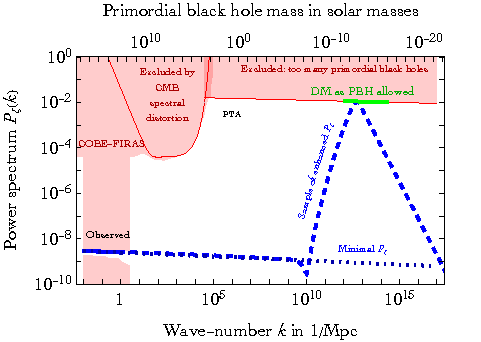
\includegraphics[width=0.65\textwidth]{figs/PowerSpectrumPBH}$$
\caption[Power spectrum for PBH]{\em  \label{fig:PowerSpectrumPBH} 
The blue curve shows the power spectrum $P_\zeta (k) \approx 2.1\, 10^{-9}$ observed on cosmological scales, $k  \lesssim 1/{\rm Mpc}$.
The DM abundance is reproduced as Primordial Black Holes if $P_\zeta$ grows up to  $\sim 10^{-2}$ around the green region,
as exemplified by the dashed curve.
The shaded red regions are excluded by the CMB $\mu$-distortions and by a too large PBH abundance that would result in a DM abundance above the observed one~\cite{2008.03289}.
}
\end{figure}


\medskip

Primordial black holes would have formed out of ordinary collisional matter, without the need for extra DM particles, 
if the primordial matter density inhomogeneities at the appropriate scales were large, $\delta_k \circa{>} 1$. This is still possible for scales $1/k$ that are much smaller than those
being probed by the current cosmological observations.
Gravitational collapses of roughly spherical over-dense regions would then lead to the creation of black holes.

One of the primary quantities of interest is the mass distribution of primordial black holes.
When a large primordial inhomogeneity on a scale $k$  re-enters the horizon, 
$k \sim aH$, it produces black holes 
with a typical mass comparable to the total mass contained within the horizon.
This happens at a temperature $T \sim k M_{\rm Pl}/T_0$, which follows immediately from $k \sim aH$, using
the Hubble rate
$H \sim T^2/M_{\rm Pl}$, as appropriate for the radiation-dominated era, $T \circa{>} 10^3\, T_0$, and then inserting $T \sim T_0/a$.
Since the horizon radius was $R\sim 1/H$ and the cosmological density was $\rho \sim T^4$, the typical black hole mass is
\beq \label{eq:MBHT}
M \sim \rho R^3 \sim \frac{M_{\rm Pl}^2}{H}\sim
 \frac{M_{\rm Pl}^3}{T^2} \sim \frac{M_{\rm Pl} T_0^2}{k^2} .
 \eeq
The expression in terms of $H$ can, equivalently, also be derived from the Schwarzschild radius $R\sim GM$.
Numerically, one obtains 
\beq 
M \sim 10^{15} \, {\rm g} \left(\frac{t}{10^{-23} \, {\rm s}}\right) \sim 2 \, M_\odot \left( \frac{{\rm GeV}}{T} \right)^2 \sim 250 \, M_\odot \left( \frac{10^5 \, {\rm Mpc}^{-1}}{k} \right)^2.
 \eeq
The relation \eqref{eq:MBHT} is used in fig.\fig{PowerSpectrumPBH} to link the PBH mass $M$ (upper horizontal axis)
to the scale $k$ (lower axis). 
A few illustrative numerical examples are as follows:
\begin{itemize}
\item[$\circleddash$] If gravitational collapse occurred at a temperature near the QCD phase transition,
$T\sim \Lambda_{\rm QCD} \sim m_p$, 
the scale entering the horizon would be $k \sim 1/{\rm pc}$.
This would result in the formation of PBHs with masses comparable to the Chandrasekhar limit,
$M \sim M_{\rm Pl}^3/m_p^2 \sim M_\odot$, i.e., of the order of the solar mass.

\item[$\circleddash$] 
A collapse occurring just before BBN, at a temperature $T\gtrsim  \MeV$, 
would result in PBHs whose masses are comparable to those of super-massive BHs found
at the centers of present day galaxies, $M\sim 10^5 \, M_\odot$.

\item[$\circleddash$]  
At the other extreme, the formation of PBHs at the Planck temperature leads to black holes with Planck masses $M \sim M_{\rm Pl}\sim 10^{-5}$\,g, which then quickly evaporate away.\footnote{Small primordial black holes could be relevant for DM in a different, indirect way: their evaporation could produce DM particles~\cite{DMfromPBH}.\index{Primordial black holes!producing particle DM}
}
\item[$\circleddash$]  
Finally, the PBHs in the asteroid mass range, where PBHs could be all of the DM (see section \ref{MACHO}),
would be formed at temperatures $T \sim{\rm PeV}$.
\end{itemize}
The observed DM abundance is reproduced if the fraction of the total cosmological
density that collapses into primordial black holes
equals  $\wp \sim T_0/T \sim 10^{-18}$ (similarly to eq.\eq{YDM0}).
It can be even smaller, if the BHs later accrete significant amounts of matter.

\smallskip
The fraction $\wp$ of the total mass that collapses into black holes can be computed in terms of
$\delta_k$ along the lines of section~\ref{sec:haloMf},
obtaining a result similar to eq.\eq{pcollapse}.
From it one can find that the typical inhomogeneity $\sigma_R \sim \delta_k \gg 10^{-5}$ needs to be enhanced
up to $\sim 10^{-2}$,
as illustrated in fig.\fig{PowerSpectrumPBH} in terms of the power spectrum $P_\zeta \sim \sigma_R^2$.
The required small $\wp \ll 1$ is obtained from exponentially rare regions with
over-densities large enough that the PBHs are produced.
Thereby the PBH abundance is exponentially sensitive to the parameters of the particular model,
and models mostly tend to predict a narrow peak in the PBH mass distribution,
as well as clusters of nearby primordial black holes~\cite{PBHclustering}.
Note also that eq.\eq{pcollapse} was computed in the Gaussian approximation, 
while the small-scale fluctuations relevant for the PBH production could be non-Gaussian.


\smallskip

In the following we discuss specific mechanisms
that could lead to the large inhomogeneities on small scales that are required for efficient PBH production.




\begin{figure}
\begin{center}
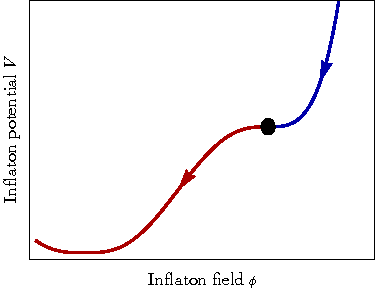
\includegraphics[width=0.45\textwidth]{figs/PotentialInflectionPoint}\qquad
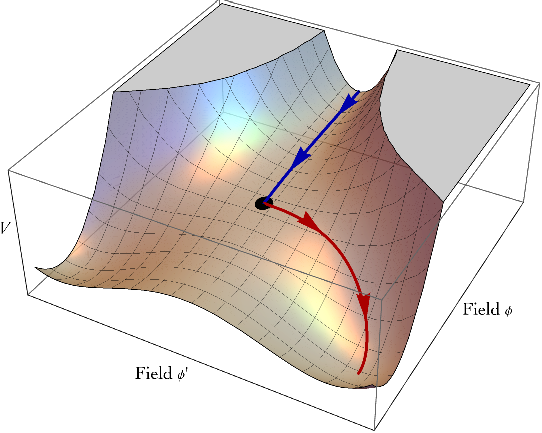
\includegraphics[width=0.45\textwidth]{figs/WaterFallInflationV}
\caption[Water-fall potential]{\em  Sample inflaton potentials that generate large inhomogeneities
around the black dot along the inflationary trajectory.
{\bfseries Left}: one-field potential with an inflection point. 
{\bfseries Right}: two-field water-fall hybrid inflation.
\label{fig:WaterFallInflationV}}
\end{center}
\end{figure}


\subsection{Primordial black holes from enhanced inflationary perturbations}\label{sec:BHth}
\index{DM theory!primordial black holes}\index{Primordial black holes!formation}\index{Black hole!formation}
The small primordial inhomogeneities observed on cosmologically large  scales are 
usually interpreted as imprints of quantum fluctuations during inflation, as discussed in section \ref{sec:linear:inhom}.
As illustrated in fig.\fig{PowerSpectrumPBH}, the same inflationary mechanism could, in principle, produce large inhomogeneities on small scales, which collapse and generate PBHs. 

As discussed in the previous section, PBHs form when the typical length scale of the large
inhomogeneity matches the size of the Universe (i.e., the inhomogeneities on length scale $1/k$ re-enter the horizon). 
This occurs at some temperature $T$, and the corresponding Hubble rate $H$ then determines the resulting PBH mass via eq.\eq{MBHT}.
In the inflationary case under discussion, the horizon re-entering happens at
$H \sim H_{\rm infl} \, e^{-2N}$, where $H_{\rm infl}$ is the Hubble constant during inflation and $N$ is the number of $e$-folds before the end of inflation. The corresponding temperature is $T \sim T_{\rm RH} e^{-N}$, where $T_{\rm RH} \sim \sqrt{M_{\rm Pl} H_{\rm infl}}$ is the reheat temperature (the temperature up to which the Universe reheats after the end of inflation).
The above relations take into account that the scale factor expands exponentially during inflation, $a \propto e^{N}$,
and the universe cools as $T \propto 1/a$ after inflation.
Inserting this into eq.\eq{MBHT} shows that the typical PBH mass is
\beq 
M \sim \frac{M_{\rm Pl}^2}{H_{\rm infl}} \, e^{2N}. 
\label{eq:MPBHN}
\eeq
Assuming $H_{\rm infl}\sim 10^{14}$ GeV, eq.\eq{MPBHN} then implies that the PBHs that have the mass in the observationally allowed range for them to be all of DM, 
$M \sim 10^{-12-16} M_\odot$, eq.\eq{PBH},
need to be seeded roughly $N\sim 20$ $e$-folds  before the end of inflation 
(that is, roughly $\sim 30$ $e$-folds after the creation of cosmological inhomogeneities from quantum fluctuations).

\medskip

This mechanism is testable.
The power spectrum $P_\zeta(k)$ of primordial inhomogeneities
unavoidably produces,
at second order in cosmological perturbation theory,
the so called  Scalar Induced Gravitational Waves (SIGW) spectrum of gravitational waves, centered 
at present-day 
frequency $f=2\pi k$ and with energy density~\cite{SIGW}
\beq \Omega_{\rm GW} \equiv \frac{1}{\rho_{\rm tot}}
\frac{d\rho_{\rm GW}}{d\ln f}
\sim 10^{-5} P_\zeta^2.\eeq
Inhomogeneities on small-scales large enough 
to seed primordial black holes in the DM allowed range, 
imply gravitational waves with Hz-scale frequency
and energy density $\Omega_{\rm GW} \sim 10^{-9}$:
a signal testable by  future experiments such as {\sc Lisa}.

\medskip

Which inflationary models lead to a nontrivial, scale dependent, primordial inhomogeneities, such as the example in fig.\fig{PowerSpectrumPBH}?
Minimal inflation  predicts a nearly scale-independent spectrum of primordial inhomogeneities (in agreement with data, though probed in a limited range of $k$ values, see solid and dotted blue lines in fig.~\ref{fig:PowerSpectrumPBH}).
Non-minimal  theories of inflation are therefore needed in order to have large primordial inhomogeneities on small scales (at large values of $k$), and small inhomogeneities on large scales (at small values of $k$).

Large inhomogeneities arise when quantum fluctuations become almost
comparable to the classical evolution of the inflaton field.
This can happen, if quantum effects get large\footnote{This happens at super-Planckian field values, which, however, leads to eternal inflation.},
or if classical effects get small.
The latter is realised if the inflation potential has a feature that slows down the inflaton $\phi$,
leading to an {\em ultra-slow roll} phase during which inhomogeneities
$P_\zeta \approx V/24\pi^2 \bar{M}_{\rm Pl}^4\epsilon$ are enhanced by the ultra-small parameter
$\epsilon = (d\phi/dN)^2/2\bar{M}_{\rm Pl}^2$.
The power spectrum can be computed precisely by solving for
the evolution of the quantum modes $\delta \phi_k$ of the inflaton. The computation is simplified, if one uses the
coordinate-independent combination
$\zeta_k = -\Psi_k +  \delta\phi_k/\dot\phi$, where $\Psi$ is the gravitational potential of eq.\eq{metricPhiPsi}.
The curvature perturbation $\zeta$ indicates the spatial curvature of surfaces of constant $\phi$.
The $k-$Fourier mode of curvature perturbation, $\zeta_k$, 
determines the power spectrum at late times as $P_\zeta(k) = k^3 |\zeta_k|^2/2\pi^2$,
and evolves following the Mukhanov-Sasaki equation~\cite{MS}
\beq \label{eq:MS2}
\frac{d^2 \zeta_k}{dN^2}+ (3+ \epsilon- 2\eta) \frac{d\zeta_k}{dN} + 
\frac{k^2}{a^2 H^2} \zeta_k=0,\qquad \eta = \epsilon - \frac{1}{2} \frac{d}{dN}\ln \epsilon.
\eeq
Amplification happens for  $3+ \epsilon- 2\eta<0$, 
which can be satisfied during an ultra-slow roll  phase with large $\eta \gtrsim 1$.
Examples of features in the potential that lead to an amplification are an {\em especially flat} region 
such as an approximate plateau, an {\em inflection point} (either exact with $V'=0$, or approximate with small $V'$),
a {\em little bump} in the inflation potential that slows downs or possibly mildly traps the inflaton,
or {\em enhanced dissipative friction}~\cite{PBHformationTh,HiggsPlateau}.

In models with a single inflaton field, the required ultra-flat potential can be achieved via tuning of parameters or by assuming a pole in the inflaton kinetic term~\cite{PBHformationTh,HiggsPlateau}.
Extreme flatness naturally arises in {\em `hybrid inflation'} models with two scalars $\phi$ and $\phi'$, if the potential has the {\em `water-fall'} form.
Namely, we can assume that initially $\phi'=0$ because its 
field-dependent squared mass $m_{\phi'}^2(\phi)$ is positive for initial values of $\phi$,
and that the $m_{\phi'}^2(\phi)$ turns negative at some critical value $\phi_*$.
As illustrated in fig.\fig{WaterFallInflationV}, at this point the potential is extremely flat along the $\phi'$ direction, and a phase transition happens.
In general, phase transitions  can be induced during inflation by the time-dependence of the inflaton field,
 and can thus also proceed in the reverse order (i.e., from a broken phase at early times to an unbroken phase at later times).
For instance, the symmetry that keeps light some additional `curvaton' field might get restored during later stages of inflation.
The `water-fall' model provides a specific realization of a quite general idea of {\em`double inflation'}, i.e., two separate periods of inflation,
which generate different amounts of inhomogeneity, and on different scales.

\smallskip

A different possibility is a {\em sharp step-like feature} in the quasi-flat inflaton potential
or a {\em dip}. In this case, the sudden acceleration makes  the slow-roll parameter $\eta$ temporarily
large, mildly enhancing fluctuations~\cite{PBHformationTh}.
A larger effect can arise from a few consecutive steps or dips.
Yet another possibility is that the inflaton fragments into localised solitons, termed {\em `oscillons'}~\cite{PBHformationOscillon}.
An attempt at producing the PBHs within the SM Higgs inflation is discussed in section~\ref{sec:PBHSM}.


In most of these models an enhancement of $P_\zeta$ by 6 orders of magnitude
needs a tuning of the model parameters with a precision of $10^{-3}$.



\subsection{Primordial black holes from first-order phase transitions}\index{Phase transitions}
\label{sec:BHth2}
An entirely different possibility is that the PBHs were created after inflation.  
This is possible, if the cosmological evolution of the early Universe included a {\em first order phase transition} at some temperature $T$,
which ended after the bubbles of the lower energy vacuum nucleated at random places and times and then expanded until the true vacuum filled the entire space.
The bubble nucleation rate per unit volume
is given by $\gamma \approx T^4 (S_3/2\pi T)^{3/2} e^{-S_3/T}$ where $S_3(T)$ is the thermal bubble action.
The nucleation happening at temperature $T$ therefore has $S_3/T\approx 4 \ln M_{\rm Pl}/T$.
As an example, a thermal potential of a scalar $\phi$ with negligible cubic, $V(\phi) \approx (g^2 T^2/12)\phi^2/2 - \lambda \phi^4/4$,
leads to $S_3/T \approx  5.4 g/\lambda$.
A first order phase transition can form PBHs via multiple mechanisms~\cite{PBHformationPhaseTransition}:
\begin{itemize}
\item[$\circledcirc$] {\bf Collisions of bubbles} generate PBHs in large enough quantities to be the DM, provided that
\beq \alpha \equiv \frac{\Delta V - d(\Delta V)/d\ln T}{g_* \pi^2 T^4 /30}\sim 1,\qquad 
 \frac{\beta}{H} \equiv  -\frac{d\ln\gamma}{d\ln T}\approx \frac{d(S_3/T)}{d\ln T}\sim 1.\eeq
The first condition demands that  the change in the energy density $\Delta V$ due to the phase transition  is an $\mathcal{O}(1)$ fraction of the total cosmological energy density.
The second condition demands that the inverse duration of the phase transition, $\beta \equiv d\ln \gamma/dt$,
is comparable to the Hubble rate at the time at which the transition happens, $\gamma \sim H^4$.
This condition is needed because a  nucleation rate that grows too fast leads to many small bubbles. 
The same bubble collisions also generate gravitational waves, which can allow to test the scenario.



\item[$\circledcirc$] {\bf Late blooming regions in super-cooled} first-order phase transitions can form PBHs in the following way.
Regions where the phase transition is completed get filled by radiation or matter, whose energy density red-shifts away.
Regions where bubbles accidentally form at a later time, become relatively denser, because their
energy density is dominated by the vacuum energy of the false vacuum, which does not red-shift away.
Denser regions can become black holes.
PBHs in the mass range where they can be the DM candidates arise, if the super-cooling starts at a temperature $T \sim 10^{4-7}\GeV$~\cite{PBHformationTh}.


 \item[$\circledcirc$] 
{\bf Matter compression}. 
If the first order phase transition occurs in the presence of a particular type of particle dark matter, which cannot easily enter bubbles of the new phase,
then the bubble expansion compresses the dark matter, forming macroscopic objects and possibly 
black holes~\cite{QballsBis}. Specific realizations of this mechanism are discussed in section \ref{sec:MacroCompositeDMth}.

 \end{itemize}

 In all of the above cases new physics is needed, since the SM does not predict any first-order phase transition.\footnote{The QCD phase transition, even though it is a cross-over, can still play a role:
the presence of many non-relativistic particles around the QCD scale implies a mildly reduced pressure (see fig.\fig{dofSM} in the appendix), which enhances the growth of  milder pre-existing inhomogeneities~\cite{PBHformationTh}.
The critical density threshold $\delta_c$ for PBH formation gets reduced by about $10\%$.
This mild reduction significantly enhances the PBH formation rate because,
similarly to eq.\eq{pcollapse}, the collapsed fraction is exponentially sensitive to the density threshold for the collapse.
This effect also means that the power spectrum of primordial inhomogeneities,
which is enhanced and nearly scale-independent at small scales, 
would give a PBH spectrum peaked around the solar mass.
This effect is therefore not relevant for PBH as DM, see \arxivref{1904.02129}{Carr et al.~(2021)} in~\cite{PBHformationTh}.}

\medskip


In addition to collisions of bubbles, 
the PBHs could be formed via other similar objects that may get created during a particular phase transition, for instance cosmic strings, domain walls~\cite{PBHformationPhaseTransition} or oscillons~\cite{PBHformationOscillon}. 
Finally, PBHs might be a property of particle DM rather than an alternative to it:
one can devise models of DM particles that cluster via some attractive long-range force and lead to the creation of PBHs.



